\documentclass[fr]{../../../eplsummary}


\newcolumntype{x}[1]{>{\centering\let\newline\\\arraybackslash\hspace{0pt}}p{#1}}
\renewcommand{\it}[1]{\textit{#1}}
\renewcommand{\bf}[1]{\textbf{#1}}
\newcommand\tab[1][1cm]{\hspace*{#1}}
\usepackage{slashbox}

\hypertitle{\'{E}conomie Politique}{3}{ECGE}{1115}
{Guillaume Prieur}
{Pierre Dehez \and Rigas Oikonomou}


\part{Micro-économie}
\section{Introduction}
\subsection{Les 10 principes de Mankiw}
\noindent
\textbf{Décisions individuelles} : 
\begin{itemize}
    \item Les "agents économiques" doivent faire des choix rationnels face à des contraintes.
    \item Le coût d'un bien est ce à quoi on est prêt à renoncer pour l'obtenir. On parle de \it{coût d'opportunité}.
    \item Les individus rationnels raisonnent à la marge et sont sensibles aux incitations. La différence entre le prix et le plan d'action est la \it{variation marginale}.
\end{itemize}
\bf{Interactions entre agents économiques} :
\begin{itemize}
\item Les échanges peuvent être profitable à tous les partis.
\item Le marché permet \it{en général} une organisation efficace de l'économie.
\item L'état peut parfois améliorer les résultats du marché. Il y a un contrôle publique.
\end{itemize}
\bf{Fonctionnement globale de l'économie} :
\begin{itemize}
\item Le niveau de vie d'un pays dépend de sa capacité à produire des biens et des services.
\item Les prix tendent à augmenter lorsque l'état imprime de la monnaie. Il y a une inflation générale des prix.
\item A court terme, un compromis existe entre l'inflation et le chômage.
\end{itemize}
\subsection{Contraintes et objectifs}
\subsubsection{Contraintes budgétaires}
\noindent
On a plusieurs types de contraintes : contrainte de temps, contrainte de production, contrainte technologique, contrainte budgétaire, etc. Dans tous les cas, on a un ensemble de possibilités réalisables, il faut donc faire un \it{choix}. Ce choix résulte d'une optimisation  
\begin{figure}[ht!]
    \centering
    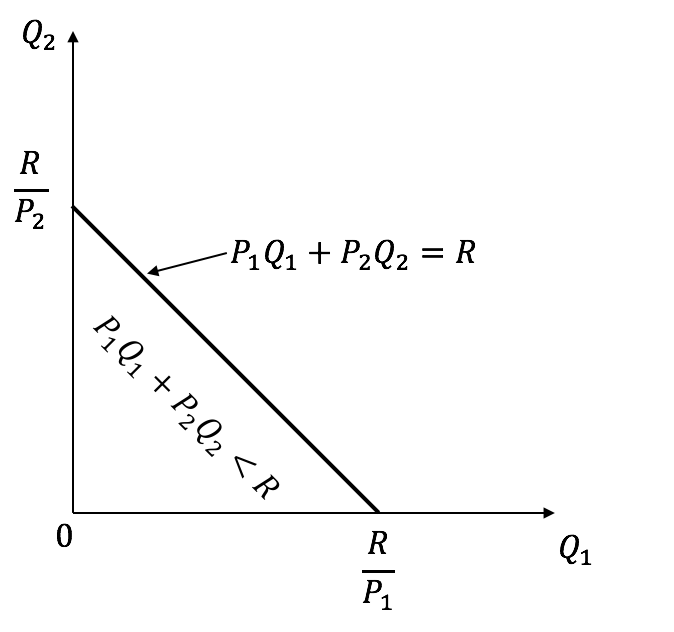
\includegraphics[scale = 0.5]{img/budget.png}
    \caption{Contrainte budgétaire avec deux biens}
    \label{budget}
\end{figure}
Dans le cas d'une contrainte budgétaire (cfr. Figure \ref{budget}), on sacrifie un bien pour augmenter l'autre. Si $R$ est le budget, et $Q$ et $P$ les quantités et les prix des biens, on a 
\begin{align}
    P_1Q_1 + P_2Q_2 = R\label{R1}
\end{align}
Grâce à l'équation \ref{R1}, on peut donner la valeur absolue de la pente $\frac{P_1}{P_2}$ qui est définie comme le \it{prix absolu}. \\
\\
Si on a une augmentation du revenu (cfr. Figure \ref{budgetplus}), le rapport de prix reste inchangé mais on a un déplacement de la contrainte budgétaire qui se fait parallèlement.\\
\\
Si on a une augmentation de prix(cfr. Figure \ref{budgetmoins}), on a une perte du pouvoir d'achat. On a
\begin{align*}
    P_2 \uparrow \Rightarrow \frac{P_1}{P_2}\downarrow
\end{align*}
\begin{figure}[ht!]
\begin{minipage}[b]{.46\linewidth}
\centering
    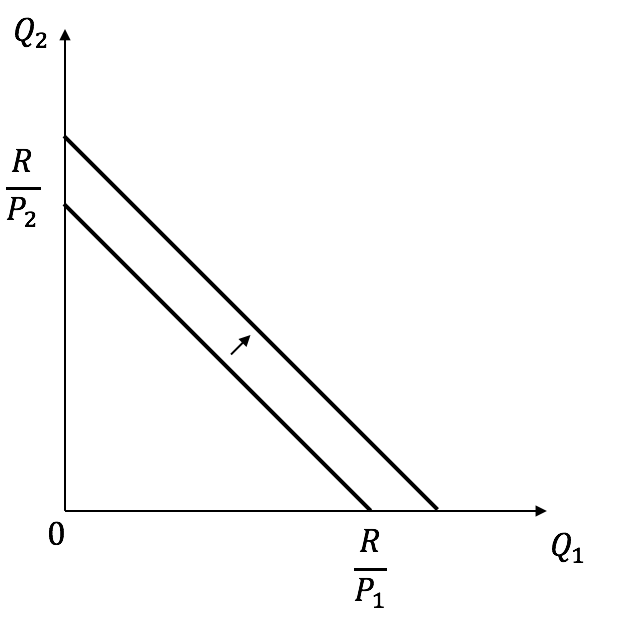
\includegraphics[scale = 0.5]{img/budgetplus.png}
    \caption{Augmentation du revenu}
    \label{budgetplus}
\end{minipage}
\begin{minipage}[b]{.46\linewidth}
\centering
    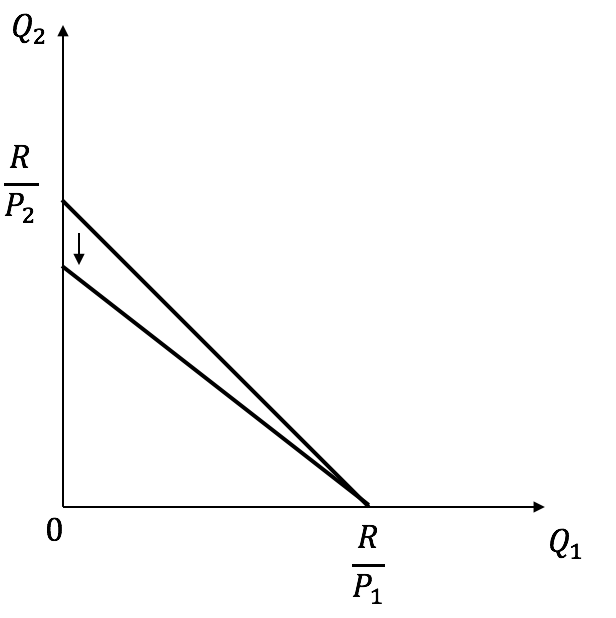
\includegraphics[scale = 0.5]{img/budgetmoins.png}
    \caption{Augmentation de prix}
    \label{budgetmoins}
\end{minipage}
\end{figure}
\subsubsection{Quelques définitions...}
\noindent
\bf{Stock} : Un stock à un instant $t$ est une quantité qui résulte d'une accumulation.\\
\bf{Flux} : Un stock varie sur une période suite à un flux (négatif ou positif).\\
\bf{Variables endogènes} : Variables appliquées par le modèle.\\
\bf{Variables exogènes} : Variables qui déterminent le modèle.
\section{Technologie}
\noindent
Une technologie est définie par un ensemble de plans de production qui sont techniquement réalisables (combinaisons d'outputs et inputs). Pour qu'un plan de production soit efficace, il faut qu'il soit impossible de
\begin{itemize}
    \item produire plus d'un bien sans réduire la production d'autres et/ou d'augmenter l'utilisation de certains inputs,
    \item réduire l'utilisation d'un input sans devoir réduire la production de certains biens et/ou augmenter l'utilisation d'autres inputs.
\end{itemize}
\subsection{Fonction de production}
\noindent
Pour construire la fonction de production, il faut formuler deux hypothèses : 
\begin{itemize}
    \item pas d'output sans input $F(0,0,...0) = 0$,
    \item si input $\uparrow$ alors output $\uparrow$ : la fonction est croissante sur son domaine.
\end{itemize}
\subsubsection{Productivité moyenne et marginale}
\noindent
\bf{Productivité moyenne} : définie par la production d'un input, elle est représentée par $PM(x) = \frac{F(x)}{x}$. C'est la pente de la droite issue de l'origine\\
\bf{Productivité marginale} : définie par une augmentation de production résultant d'une augmentation d'input, elle est représentée par $Pm(x) = \frac{dy}{dx} = F'(x)$.\\
\\
On aura toujours $PM(a) > Pm(a)$ et que $PM(0) = Pm(0)$. \\
\\
\bf{Rendement d'échelle} : 
\begin{table}[ht!]
    \centering
    \begin{tabular}{|x{5cm}|x{5cm}|x{5cm}|}
        \hline
        Rendement d'échelle décroissant & Rendement d'échelle constant & Rendement d'échelle croissant \\
        \hline
        $F(\lambda x) < \lambda F(x)$ & $F(\lambda x) = \lambda F(x)$ & $F(\lambda x) > \lambda F(x)$ \\
            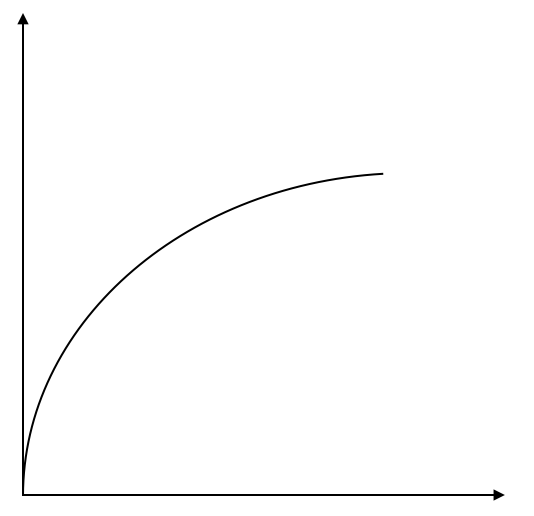
\includegraphics[scale = 0.35]{img/red1.png} &
            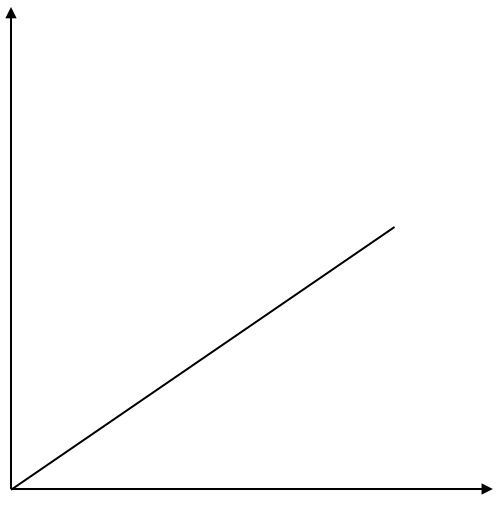
\includegraphics[scale = 0.35]{img/red2.png} &
            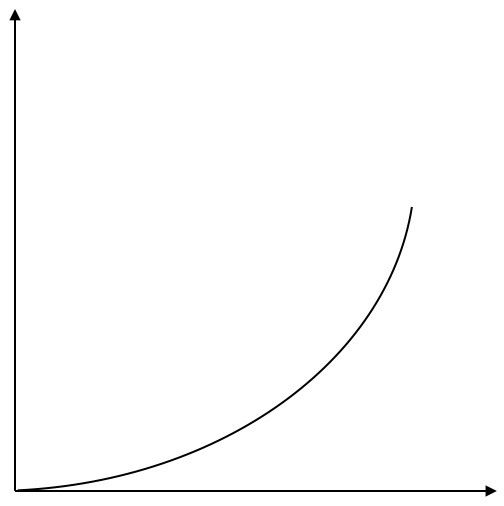
\includegraphics[scale = 0.35]{img/red3.png}\\
        $PM$ décroissant & $PM$ constant & $PM$ croissant \\
        \hline
    \end{tabular}
\end{table}
\\
Dans le cas d'un rendement mixte, la production moyenne atteint son maximum quand $PM(x) = Pm(x)$.
\subsection{Fonction de coût}
\noindent
On distingue deux types d'input :
\begin{itemize}
    \item \bf{Inputs fixes} : Ils déterminent la \it{capacité de production} ($k$) de l'entreprise. Le \it{coût fixe} $CF$ est la valeur des inputs fixes aux prix en vigueur. Il est indépendant de la quantité produite.
    \item \bf{Inputs variables} : Le \it{coût variable} $CV(q)$ est une fonction de la production $q$. C'est la dépense minimale en inputs permettant de produire $q$.
\end{itemize}
On peut alors définir la fonction de coût total 
\[CT(q) = CF + CV(q)\]
avec $0\leq q \leq k$ et $CT(0) = CF$.\\
Pour un chaîne $i$, la fonction de coût est alors donnée par
\[CT_i(q_i) = CF_i + c_iq_i\]
où $c_i = pm+wz_i$ est le coût variable avec $p$ le prix des matières premières, m la quantité de matière première, $w$ le prix de la main d'oeuvre, et $z_i$ un besoin en main-d'oeuvre par heure.\\
\\
\newpage
\noindent
Sous l'hypothèse que 
\[Z_1<Z_2<Z_3<Z_4 \Rightarrow c_1<c_2<c_3<c_4 \]
la fonction de coût peut s'écrire
\begin{align*}
    CT(q) & = CF+c_1q \quad && \text{si } 0\leq q\leq k\\
    & = CF + c_1k+c_2(q-k) \quad && \text{si } k\leq q\leq 2k\\
    & = CF + c_1k+c_2k+ c_3(q-2k) \quad && \text{si } 2k\leq q\leq 3k\\
    & = CF + c_1k+c_2k+ c_3k+ c_4(q-3k) \quad && \text{si } 3k\leq q\leq 4k
\end{align*}
où $CF$ est le coût fixe de l'ensemble des chaînes de montage.\\
Ce coût variable est toujours représenté par une courbe convexe faite d'une succession de droites parce que l'entreprise va privilégier les équipements et les compétences les moins coûteuses. 
\subsubsection{Coût total moyen et coût marginal}
\noindent
On définit 
\begin{itemize}
    \item \bf{Coût total moyen} : $CTM(q) = \frac{CF + CV(q)}{q} = CFM(q) + CVM(q) = \frac{CT(q)}{q}$
    \begin{align*}
        \text{où } & CFM(q) = \frac{CF}{q} \text{ est le coût fixe moyen}\\
        & CVM(q) = \frac{CV(q)}{q} \text{ est le coût variable moyen}
    \end{align*}
        \item \bf{Coût marginal} : $Cm(q) = CT'(q) = CV'(q)$
\end{itemize}
On a $Cm$ qui est croissant, qui passe par le minimum de la courbe $CTM$ et coïncide avec la courbe $CVM$ à l'origine (cfr. Figure \ref{cmctm}). Soit $Cm(0) = CVM(0)$ et $Cm(q_0) = CTM(q_0)$.
\begin{figure}[ht!]
    \centering
    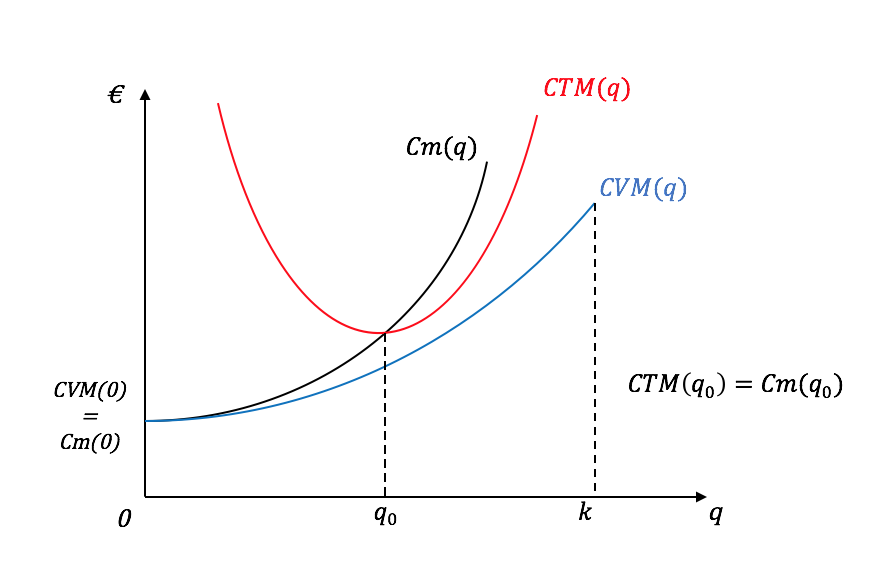
\includegraphics[scale = 0.8]{img/cmctm.png}
    \caption{Coût total moyen et coût marginal}
    \label{cmctm}
\end{figure}\\
\newpage
\noindent
\bf{Rendement d'échelle} :
\begin{table}[ht!]
    \centering
    \begin{tabular}{|x{5cm}|x{5cm}|x{5cm}|}
        \hline
        Rendement d'échelle décroissant & Rendement d'échelle constant & Rendement d'échelle croissant \\
        \hline
        Augmentation du niveau de production entraine une hausse plus que proportionnel du coût & Augmentation du niveau de production entraine une hausse proportionnelle du coût & Augmentation du niveau de production entraine une hausse moins que proportionnel du coût  \\
        $CT(\lambda q) > \lambda CT(q)$ & $CT(\lambda q) = \lambda CT(q)$ & $CT(\lambda q) < \lambda CT(q)$ \\
        \hline
        $CTM$ croissant & $CT$ est proportionnel à $q$ (absence de coût fixe) & $CTM$ décroissant \\
        $CTM(\lambda q) > CTM(q)$ & $CF = 0$ et $CT(q) = CV(q)$ & $CTM(\lambda q) < CTM(q)$\\
        \hline
    \end{tabular}
\end{table}
\section{Marchés concurrentiels}
\subsection{Typologie des biens}
\noindent
Les biens sont caractérisés par deux degrés :
\begin{itemize}
    \item \bf{Degré de rivalité} : rivalité si un bien ne peut être utilisé par deux personnes différentes.
    \item \bf{Degré d'excluabilité} : excluable si on sait contrailer la consommation.
\end{itemize}
On peut alors classer les biens tels que
\begin{table}[ht!]
    \centering
    \begin{tabular}{|c|c|c|}
        \hline
        \backslashbox{Excluabilité}{Rivalité} & 1& 0\\
        \hline
        1 &Biens privés & Biens de club\rule[-0.25cm]{0cm}{0.7cm}\\
        \hline
        0 & Ressources communes & Biens publics\rule[-0.25cm]{0cm}{0.7cm}\\
        \hline
    \end{tabular}
\end{table}
\subsection{Offre et demande}
\noindent
On distingue deux opposants dans un marché.
\begin{itemize}
\item \bf{Acheteurs} : Ils expriment une demande définie par $q_D = D(p)$. Ils définissent un prix maximum $p_a$ au quel ils sont prêt à payer pour acquérir le bien. Donc, $p<p_a$ et il réalisera un gain égal à $p_a - p$
\item \bf{Vendeurs} : Ils expriment une offre définie par $q_S = S(p)$. Ils définissent un prix minimum $p_v$ au quel ils sont prêt à céder le bien. Donc, $p_v<p$ et il réalise un gain égal à $p-p_v$.
\end{itemize}
On sait que le prix sera toujours compris entre $p_v$ et $p_a$ et le prix d'équilibre est unique :
\[D(p) = S(p) = q\]
On parle de fonction d'offre et de fonction de demande. 
\subsection{Déterminants de l'offre et de la demande}
\noindent
Les déterminants endogènes sont le prix et les quantités échangées. Les déterminants exogènes sont quant à eux variables en fonction de l'offre ou de la demande. 
\begin{itemize}
\item \bf{Déterminants exogènes de la demande} : les revenus, les préférences, les prix des biens "proches", la démographie, l'incertitude.
\item \bf{Déterminants exogènes de l'offre} : la technologie, les ressources primaires et leurs prix, le capital physique, les prix des facteurs de production, l'incertitude.
\end{itemize}
Des changements les déterminants de l'offre et de la demande entraînent des déplacements de leurs courbes (cfr. Figure \ref{dod}).
\begin{figure}[ht!]
    \centering
    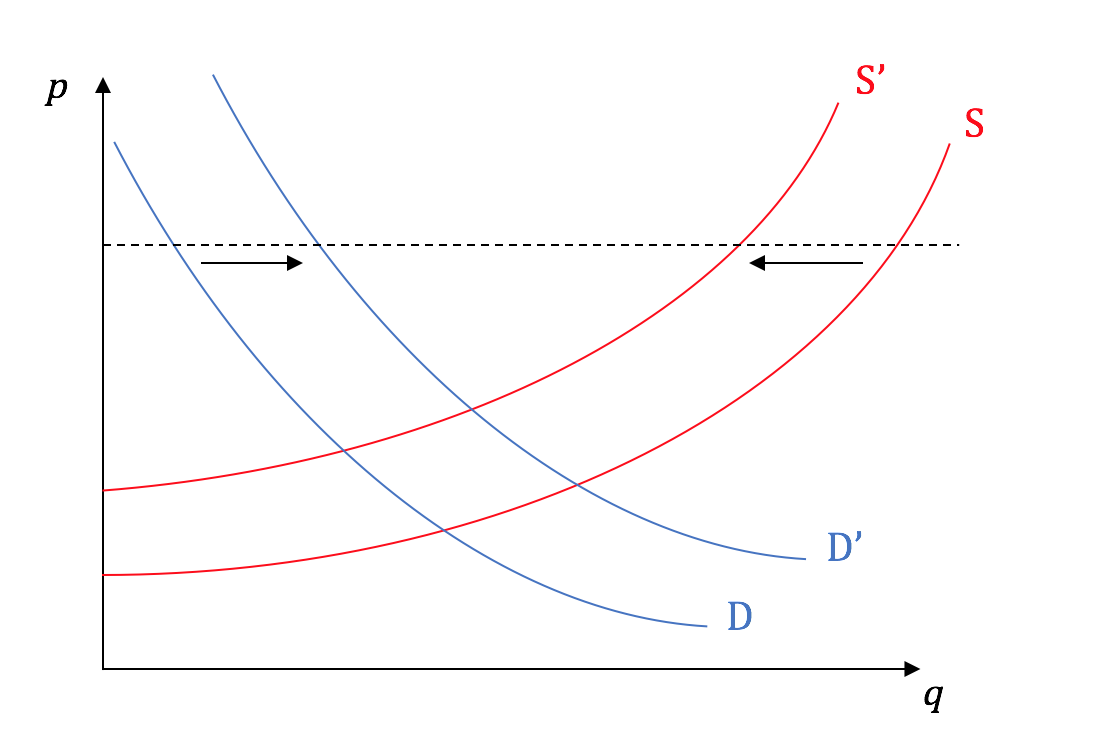
\includegraphics[scale = 0.5]{img/dod.png}
    \caption{Déplacement des courbes d'offre et de demande}
    \label{dod}
\end{figure}\\
\\
On retrouve quatre cas :
\begin{table}[ht!]
    \centering
    \begin{tabular}{|x{3cm}|x{3cm}|x{3cm}|}
        \cline{2-3} \multicolumn{1}{c|}{} & Offre & Demande\rule[-0.35cm]{0cm}{1cm}\\
        \hline
        Augmentation & $p\downarrow$ \& $q\uparrow$ & $p\uparrow$ \& $q\uparrow$\rule[-0.35cm]{0cm}{1cm}\\
        \hline
        Diminution & $p\uparrow$ \& $q\downarrow$ & $p\downarrow$ \& $q\downarrow$\rule[-0.35cm]{0cm}{1cm}\\
        \hline
    \end{tabular}
\end{table}
\subsection{Déséquilibre et ajustement}
\noindent
On retrouve deux cas de déséquilibre : excédent de demande si $p<p_\text{équilibre}$ ou excédent d'offre si $p>p_\text{équilibre}$.
\begin{table}[ht!]
    \centering
    \begin{tabular}{|x{8cm}|x{8cm}|}
    \hline
    Excédent de demande & Excédent d'offre\rule[-0.25cm]{0cm}{0.7cm}\\
    \hline
    $ED(p_0) = D(p_0)-S(p_0)$ & $ES(p_0) = S(p_0) - D(p_0)$\\
    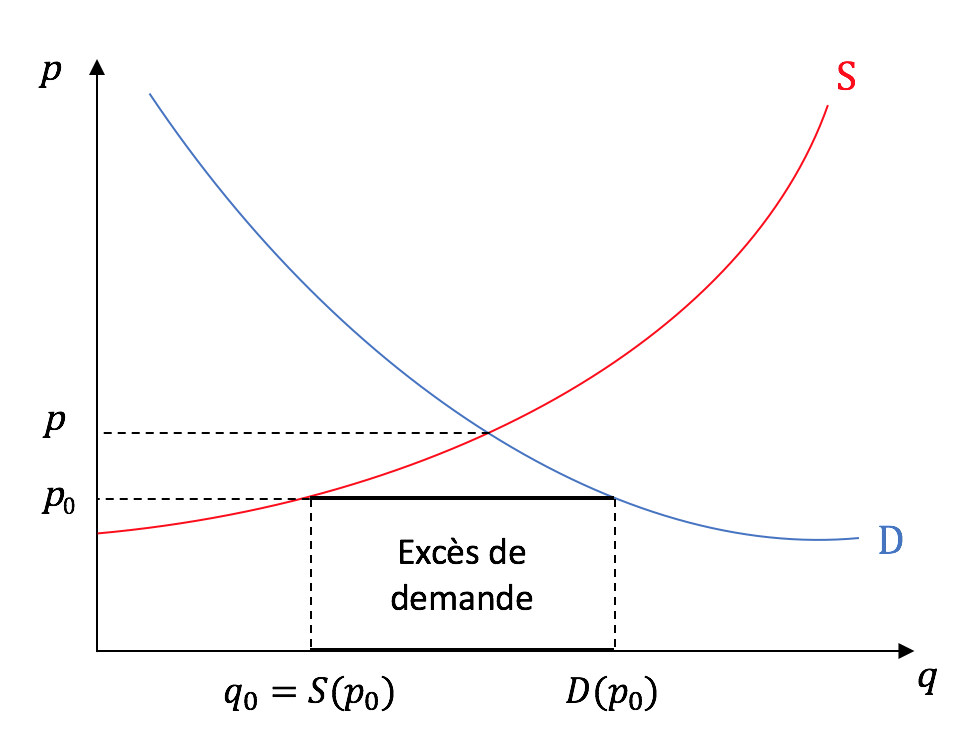
\includegraphics[scale = 0.45]{img/ed.png} & 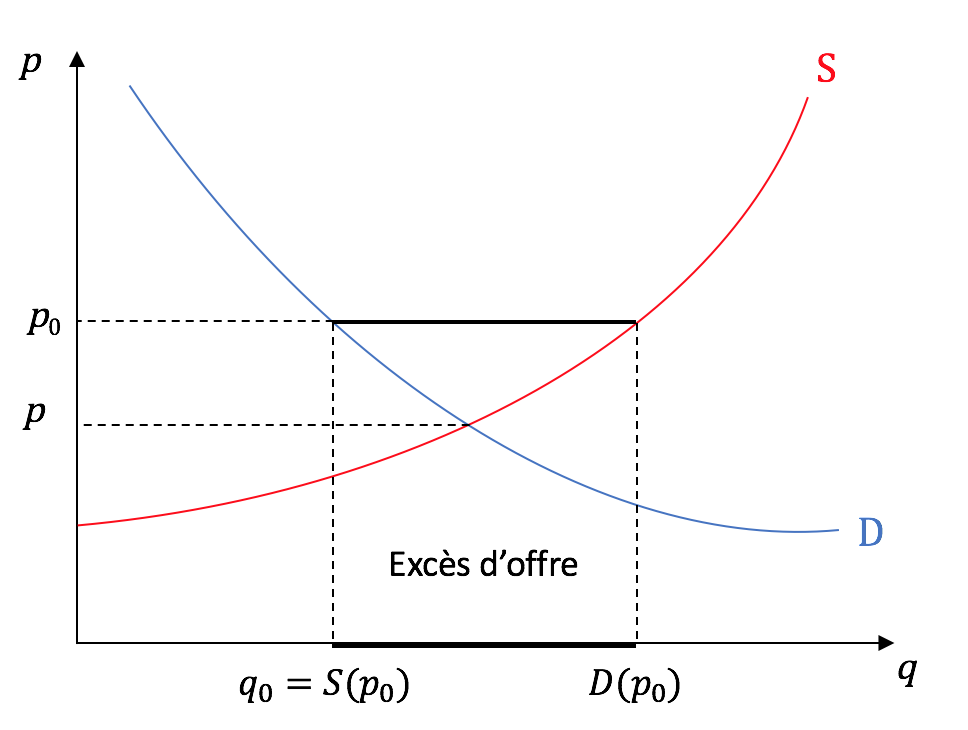
\includegraphics[scale = 0.45]{img/eo.png}\\
    Les acheteurs ont une demande insatisfaite et sont prêts à payer plus. On a un glissement du prix vers le haut. & Les vendeurs se retrouvent avec des invendus et sont prêts à vendre moins cher. On a un glissement du prix vers le bas.\\
    \hline
    \end{tabular}
\end{table}\\
\newpage
\noindent
Le mécanisme d'ajustement tend à amener progressivement le prix vers le prix d'équilibre.
\subsection{Maximisation du surplus}
\noindent
Un surplus est maximum au prix d'équilibre. Il n'y a alors aucune perte de gains.
\begin{figure}[ht!]
    \centering
    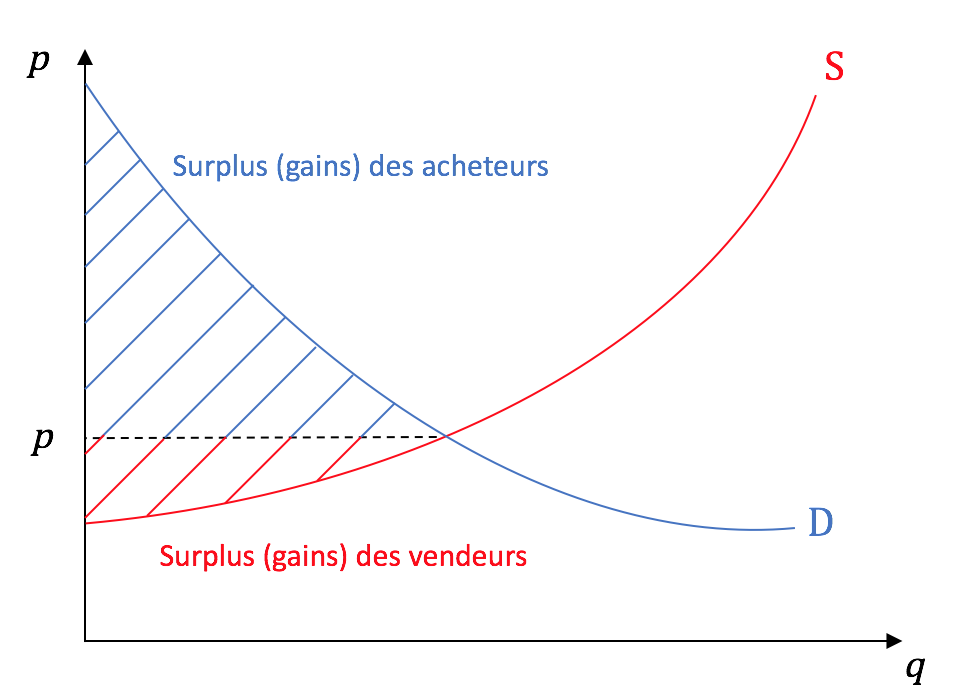
\includegraphics[scale = 0.6]{img/surplus.png}
    \caption{Déplacement des courbes d'offre et de demande}
    \label{dod}
\end{figure}\\
Si le prix n'est pas à son équilibre, on a une perte de surplus et 
\begin{itemize}
\item $p>p_\text{équilibre}$ : avantage aux vendeurs,
\item $p<p_\text{équilibre}$ : avantage aux acheteurs.
\end{itemize}
\subsection{Elasticité}
\noindent
L'élasticité est définie comme le rapport de variations relatives de deux variables liées l'une à l'autre ou le rapport de variation entre $x$ et $y$ pour $y=f(x)$.
On peut l'écrire comme
\[\varepsilon(x_0) = \frac{x_0}{y_0}\left.\frac{df}{dx}\right|_{x=x_0} = \frac{x_0}{y_0}f'(x_0)\]
On distingue deux types d'élasticité :
\begin{itemize}
\item \bf{Elasticité-prix de la demande} : est le rapport entre la variation relative de la demande d'un bien et la variation relative du prix de ce bien. Ce rapport est généralement négatif car lorsque le prix augmente, la quantité demandée diminue et réciproquement. On peut la définir comme 
\[\varepsilon_p(p) = -\frac{\frac{dp}{q}}{\frac{dp}{p}}=-p\frac{D'(p)}{D(p)}>0\]
\item \bf{Elasticité-quantité de la demande} : est l'inverse de l'élasticité-prix. On peut la définir comme 
\begin{align*}
    \varepsilon_q(p) & = -\frac{\frac{dp}{p}}{\frac{dp}{q}}=-q\frac{P'(q)}{P(q)}>0\\
    & = \frac{1}{\varepsilon_p}
\end{align*}
\end{itemize}
\subsubsection{Recette}
\noindent
La recette totale est définie par $R(p) = pD(p)$. On peut alors définir la recette marginale qui est donnée par 
\[R'(p) = D(p)+pD'(p) = D(p)\left[1-\varepsilon_p(p)\right]\]
On en déduit que la recette augmente quand $\varepsilon_p(p)<1$ et diminue quand $\varepsilon_p(p)>1$. Elle est maximal lorsque $\varepsilon_p(p)=1$.
\subsection{Interventions sur les marchés}
\noindent
Comme énoncé dans les dix principes de Mankiw, l'état a un contrôle publique.
\subsubsection{Contraintes sur les prix}
\noindent
L'Etat peut décider d'intervenir en agissant sur les prix, ce qui entraîne un déséquilibre. Il peut fixer un prix maximum (plafond) ou minimum (plancher).
\begin{table}[ht!]
    \centering
    \begin{tabular}{|x{8cm}|x{8cm}|}
    \hline
    Prix plancher &Prix plafond\rule[-0.25cm]{0cm}{0.7cm}\\
    \hline
    Le prix est minimum est alors supérieur au prix d'équilibre, ce qui crée un excédent d'offre. & Le prix maximum est alors inférieur au prix d'équilibre, ce qui crée un excédent de demande.\\
    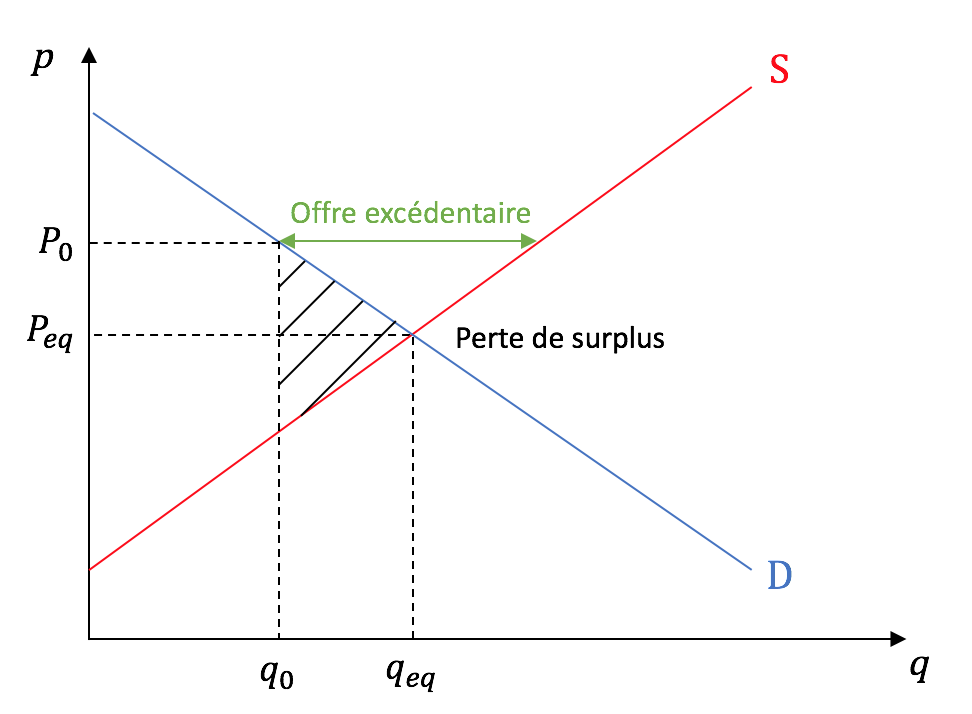
\includegraphics[scale = 0.48]{img/ppmoins.png} & 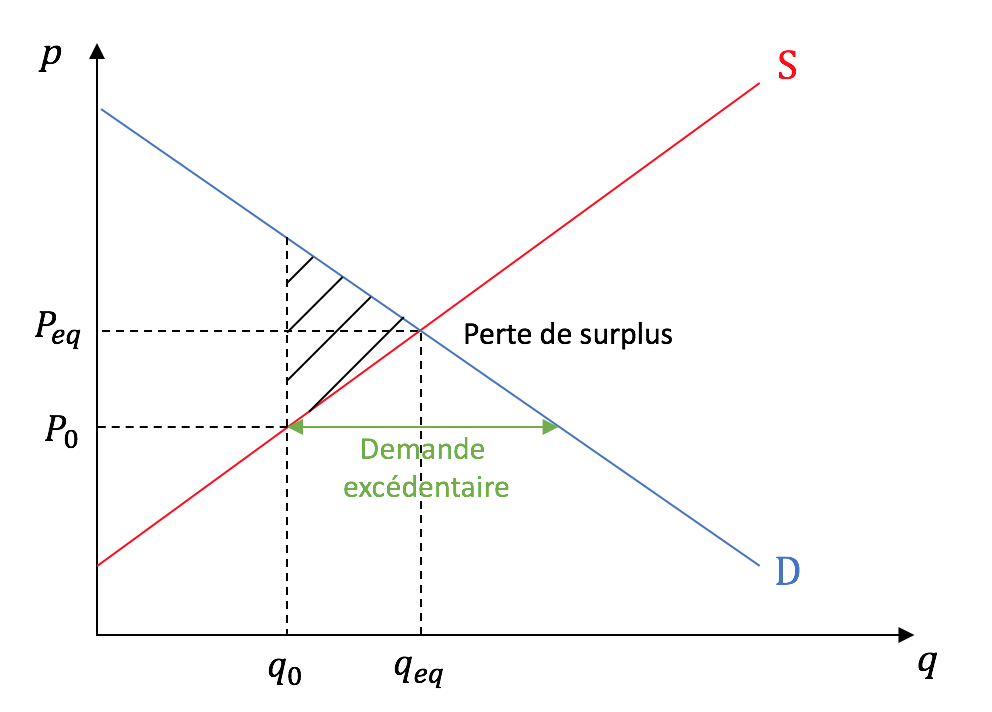
\includegraphics[scale = 0.48]{img/ppplus.png}\\
    $D(p_0)<S(p_0)$ & $D(p_0)>S(p_0)$\\
    \hline
    \end{tabular}
\end{table}\\
\newpage
\subsubsection{Introduction d'une taxe}
\noindent
L'état peut introduire une taxe unitaire et/ou un subside unitaire. Notons $T$ le montant de la taxe ; nous avons $p_a = p_v + T$. Notons également $S$ le montant du subside ; nous avons $p_a = p_v + S$.
\begin{table}[ht!]
    \centering
    \begin{tabular}{|x{8cm}|x{8cm}|}
    \hline
    Taxe unitaire T &Subside unitaire S\rule[-0.25cm]{0cm}{0.7cm}\\
    \hline
    On peut définir la recette fiscale comme $(p_a-p_v)q_e = Tq_e$ où $q_e$ sont les quantités échangées. & On peut définir la dépense publique comme $|p_v-p_a|q_e = Sq_e$ où $q_e$ sont les quantités échangées.\\
    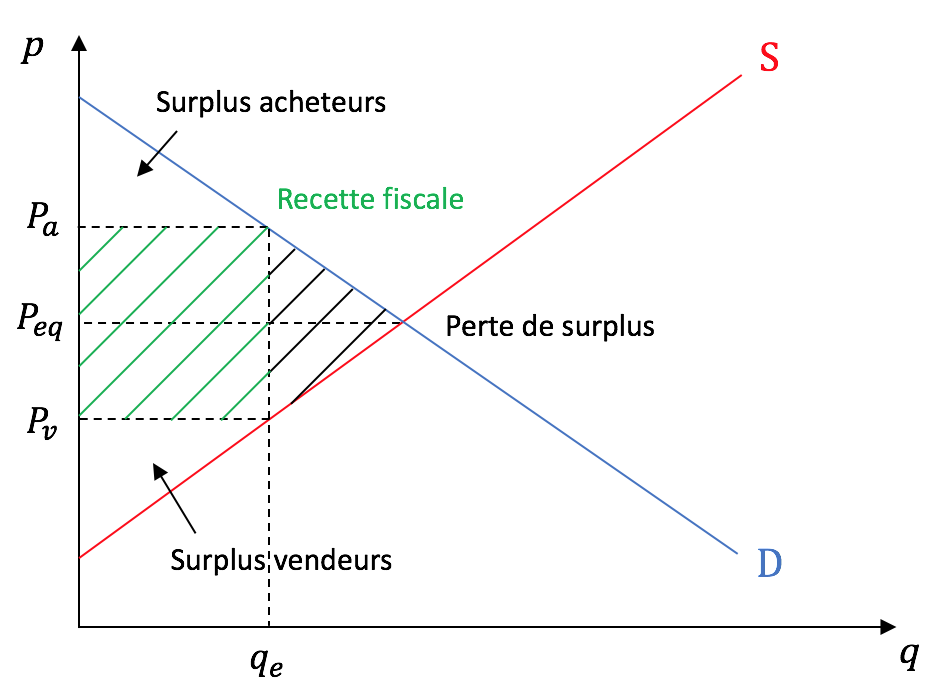
\includegraphics[scale = 0.48]{img/rf.png} & 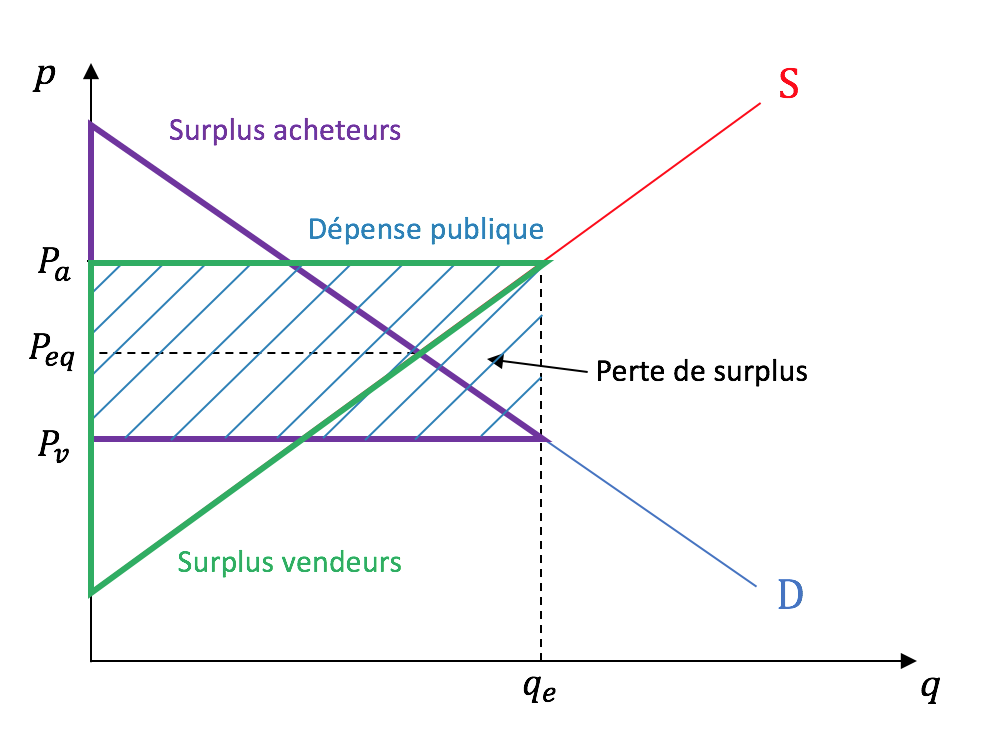
\includegraphics[scale = 0.48]{img/dp.png}\\
    \hline
    \end{tabular}
\end{table}\\
\section{Entreprises et structures de marché}
\subsection{Maximisation du profit}
\noindent
De manière générale, on écrit la recette comme une fonction de la quantité produite $R = R(q)$. On peut alors définir la recette marginale comme $Rm = R'(q)$ et le profit économique comme la différence entre la recette et le coût ou
\[\Pi(q) = R(q)-CT(q) = R(q) - CF - CV(q)\]
En raisonnant avec des petites variations de quantité produite, on peut dire que
\begin{itemize}
    \item si $Rm>Cm$, alors produire une unité de plus augmente le profit ;
    \item si $Rm<Cm$, alors produire une unité de moins augmente le profit.
\end{itemize}
La condition $Rm(q) = Cm(q)$ est donc la condition nécessaire mais pas suffisante pour la maximisation du profit.
\subsection{Concurrence parfaite}
\noindent
On considère le prix comme une donnée exogène et qu'à ce prix, l'entreprise écoulera toute sa production. On dit qu'elle est "price taker." 
La fonction de recette est donc linéaire $R(q) = pq$. Cela implique une recette marginale constante $Rm(q) = p$. La condition nécessaire de maximisation du profit s'écrit $Cm(q) = p$.\\
\subsubsection{Coût total moyen, coût marginal et profit}
\noindent
On peut maintenant améliorer notre graphique de $CTM$, $CVM$, et $Cm$ en y ajoutant la notion de profit (cfr. Figure \ref{cmctmp}). 
\begin{figure}[ht!]
    \centering
    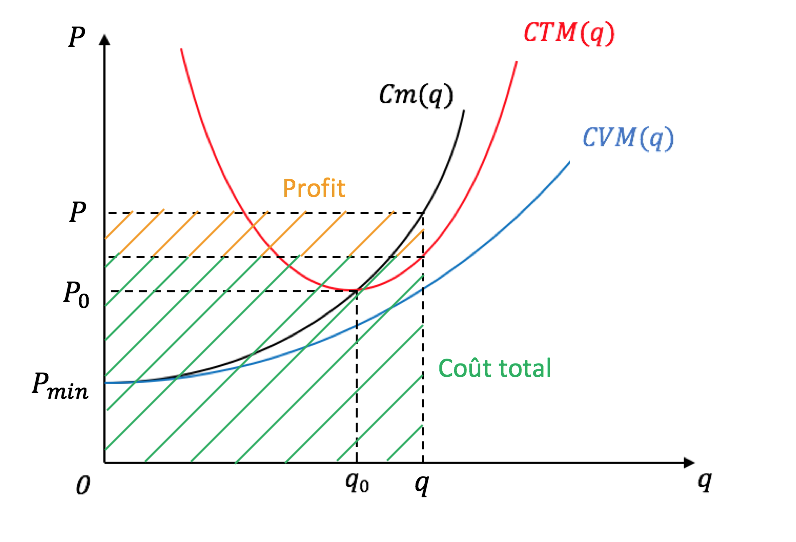
\includegraphics[scale = 0.8]{img/cmctmp.png}
    \caption{Courbes de coût marginal et coût total moyen avec profit}
    \label{cmctmp}
\end{figure}
\\
On définit notre profit comme 
\[\Pi(q) = pq-CT(q) = pq -qCTM(q) = q(p-CTM(q))\]
On retrouve trois zones de prix : 
\begin{align*}
    0 \leq p <p_\text{min} & \Rightarrow\text{ inactivité et pertes }=CF\text{ ;}\\
   p_\text{min} \leq p <p_0 & \Rightarrow\text{ pertes }<CF\text{ ;}\\
   p>p_0 & \Rightarrow\text{ profits }> 0\text{.}
\end{align*}
On définit alors deux seuils sur base de ces trois zones.
\begin{itemize}
    \item \bf{Seuil de fermeture $p_\text{min}$} : L'entreprise est indifférente entre produire et être inactive. Elle fait une perte égal à $CF$.
    \item \bf{Seuil de rentabilité $p_0$} : L'entreprise ne fait ni perte, ni profit.
\end{itemize}
Dans une perspective à long terme, il n'y a pas de coût fixe et les deux seuils coïncident puisque les courbes $CV$ et $CT$ se confondent.
\subsubsection{Offre abrégée}
\noindent
On définit l'offre abrégée comme la sommes des offres individuelles.
\subsection{Le monopole}
\noindent
L'entreprise monopolistique est seule sur le marché. Son volume de production influencera directement sur le prix du bien.
La fonction de recette s'écrit alors $R(q) =P(q)q$ et on peut en déduire la fonction de profit
\[\Pi(q) = R(q) - CT(q) = P(q)q-CT(q)\]
La fonction de recette marginal est défini comme
\[Rm(q) = \underbrace{P(q)}_{>0} + \underbrace{P'(q)q}_{<0}\]
\subsubsection{Maximisation du profit}
\noindent
La maximisation du profit s'écrit comme l'égalité du revenu marginal et le coût marginal $Rm(q)=Cm(q)$. Dans notre cas monopolistique on peut la réduire à $P(q) +P'(q)q = Cm(q)$. 
En développant cette équation, nous obtenons
\begin{align*}
    Cm(q) & = p\left( 1+\frac{dp}{dq}\frac{q}{p}\right)\\
    \varepsilon_q(p) & = \frac{p-Cm(q)}{p}
\end{align*}
On en conclut que $p>Cm$ et $\varepsilon_p>1$.
De manière générale, on mesure le pouvoir de monopole d'une entreprise par l'écart relatif entre le prix et le coût marginal
\[\mu(q) = \frac{p-Cm(q)}{p}\]
Dans le cas d'un monopole, l'égalité entre $Rm$ et $Cm$ donne
\[\mu(q) = \varepsilon_p^{-1}(q)\]
Le pouvoir du monopoleur est donc d'autant plus important que l'élasticité-prix de la demande est faible.
\subsubsection{Coût total moyen, coût marginal et profit}
\noindent
On peut tracer le graphique de $CTM$, $CVM$, $Cm$, et $\Pi$ pour un monopole.(cfr. Figure \ref{cmctmpmono}). 
\begin{figure}[ht!]
    \centering
    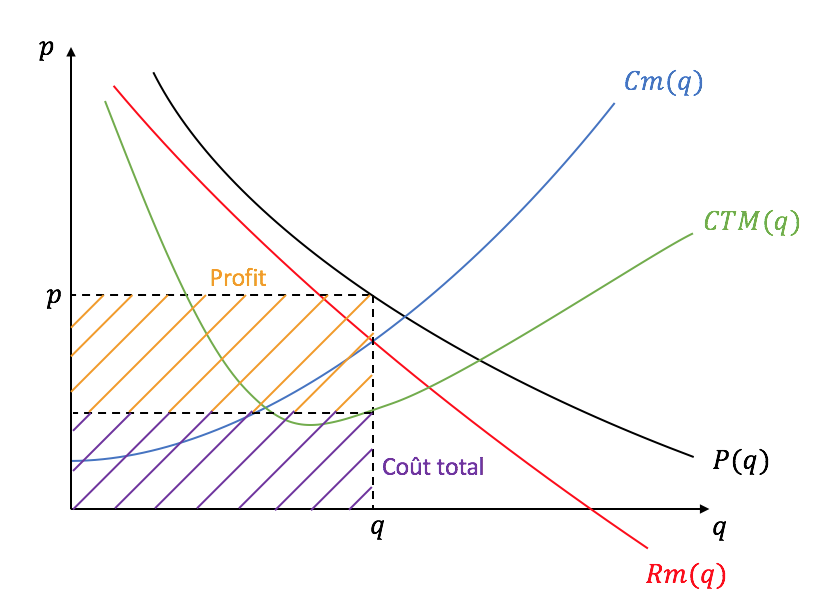
\includegraphics[scale = 0.8]{img/cmctmpmono.png}
    \caption{Courbes de coût marginal et coût total moyen avec profit pour un monopole}
    \label{cmctmpmono}
\end{figure}
\subsubsection{Le surplus}
\noindent
Lorsque le coût moyen n'est pas égal au coût marginal, nous avons que $Rm(q_m) = Cm(q_m)$ et $P(q_c) = Cm(q_c)$. Mais on a une perte de surplus pour les acheteurs (cfr. Figure \ref{s1}).
\begin{figure}[ht!]
    \centering
    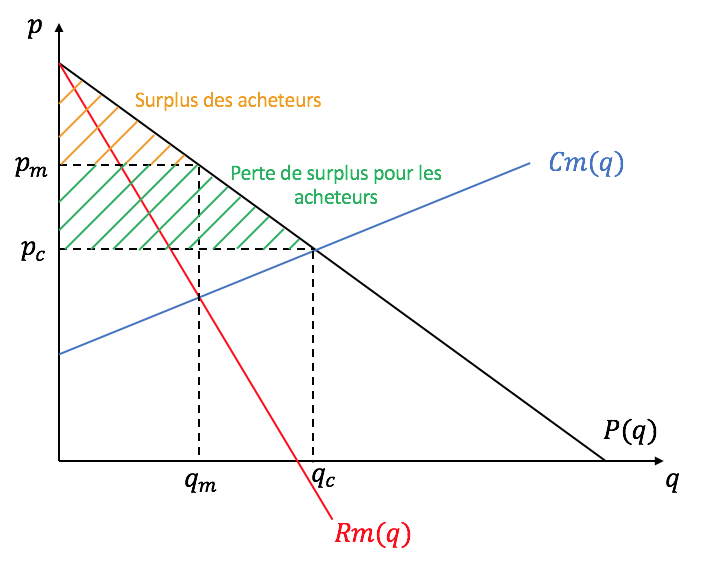
\includegraphics[scale = 0.8]{img/s1.png}
    \caption{Surplus avec un monopole}
    \label{s1}
\end{figure}
\\
Dans le cas traité par Mankiw, le coût marginal est égal au coût moyen (cfr. Figure \ref{s2}). On a un surplus "concurrentiel" $= A+M+G$ et un surplus "monopolistique" $=A+M$.
\begin{figure}[ht!]
    \centering
    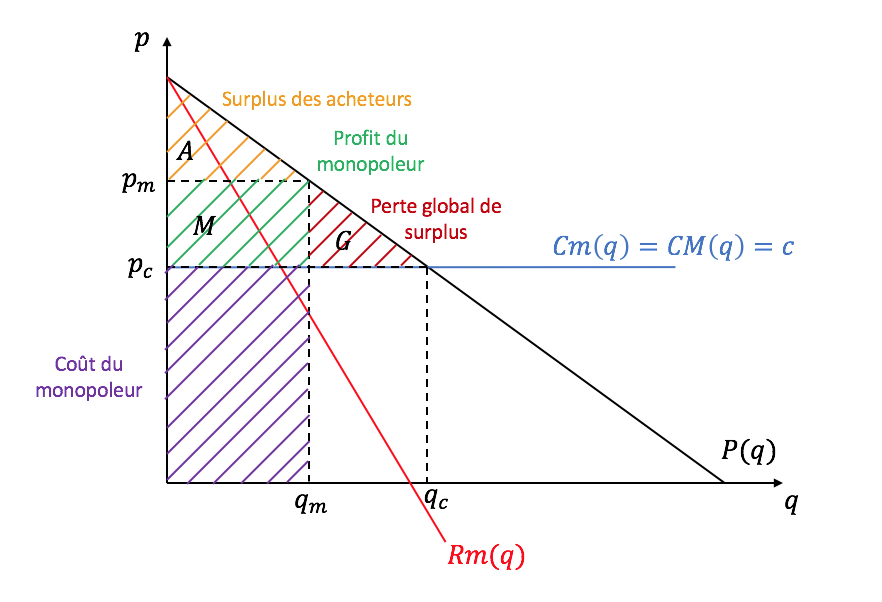
\includegraphics[scale = 0.8]{img/s2.png}
    \caption{Surplus avec un monopole selon Mankiw}
    \label{s2}
\end{figure}
\\
En pratiquant la discrimination par les prix, un monopoleur peut capturer une part plus importante du surplus des acheteurs. On a alors $p_c<p_2<p_m<p_1$. Le profit du monopoleur est alors plus élevé et égal à 
\[p_1q_1 + p_2(q_2-q_1) - cq_2\]
\subsection{L'oligopole}
\noindent
Un oligopole est une situation où quelques entreprises se disputent un même marché (cfr. Figure \ref{type}). Elles sont en interaction directe. On se limitera à deux entreprises (1 et 2) : duopole.
\begin{figure}[ht!]
    \centering
    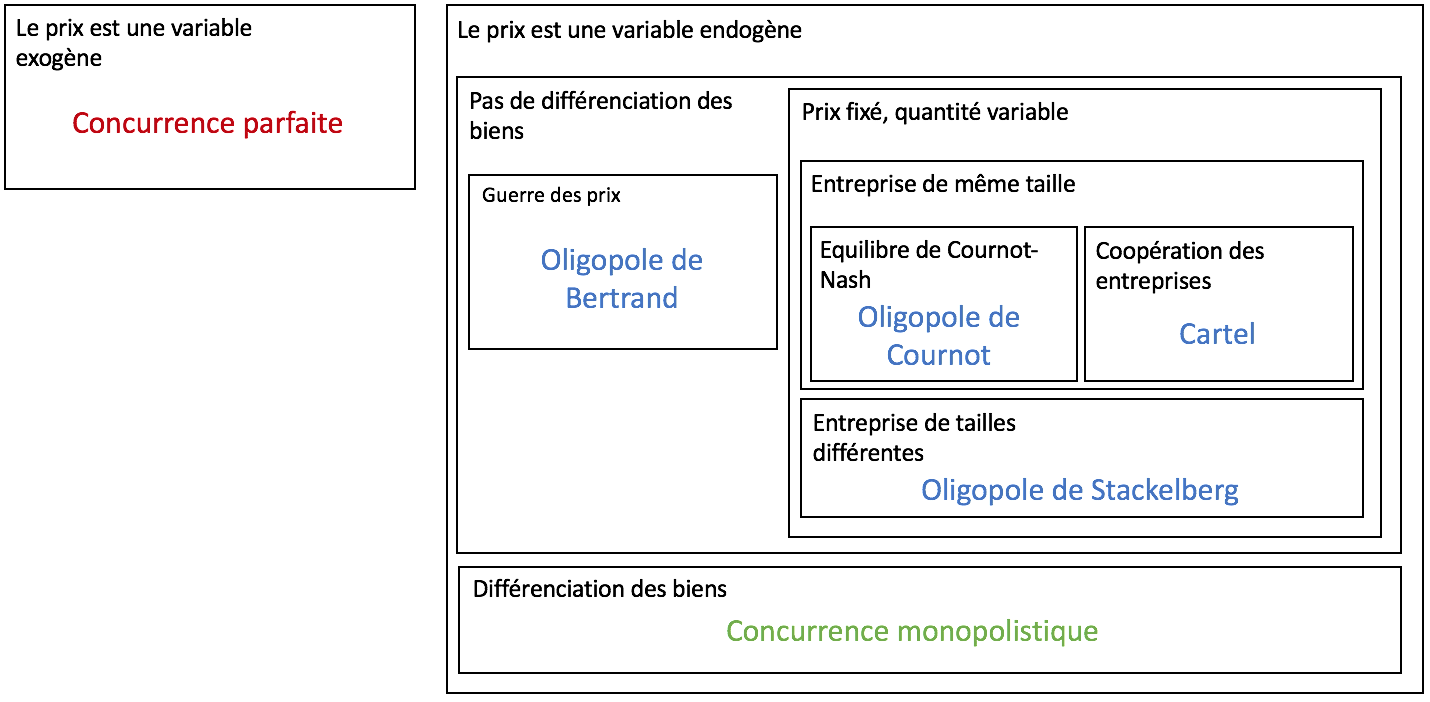
\includegraphics[scale = 0.51]{img/type.png}
    \caption{Les types de marchés en oligopole}
    \label{type}
\end{figure}
\newpage
\subsubsection{L'oligopole selon Cournot}
\noindent
On définit l'offre total comme $q = q_1 + q_2$ et donc par extension $p=P(q_1+q_2)$. On peut donc définir les profits de manière indépendante 
\begin{align*}
    \Pi_1(q_1,q_2) & = P(q_1+q_2)q_1 - C_1(q_1)\\
    \Pi_1(q_1,q_2) & = P(q_1+q_2)q_2 - C_2(q_2)
\end{align*}
Chaque entreprise cherche à maximiser son profit mais celui-ci dépend de la quantité produite par l'autre.\\
Pour résoudre ce problème, Cournot dit qu'il faut observer une situation où les quantités produites par chaque entreprise sont telles que chaque entreprise maximise son profit.
\begin{align*}
    \Pi_1(\overline{q_1},\overline{q_2}) & \geq\Pi_1(q_1,\overline{q_2}) \quad & \forall q_1 \geq 0\\
    \Pi_2(\overline{q_1},\overline{q_2}) & \geq\Pi_2(\overline{q_1},q_2) \quad & \forall q_2 \geq 0\\
\end{align*}
Aucune entreprise ne doit avoir intérêt à modifier sa stratégie. On parle d'une situation d'équilibre au sens de Cournot - Nash.\\
\\
On peut appliquer la théorie des jeux à l'oligopole de Cournot. Chaque entreprise peut calculer ce qu'elle fera en réponse à ce que fait l'autre.
\begin{itemize}
    \item $\text{Max }\Pi_1(q_1,q_2)$ par rapport à $q_1$ étant donné $q_2$ conduit à une solution $q_1 = f_1(q_2)$.
    \item $\text{Max }\Pi_2(q_1,q_2)$ par rapport à $q_2$ étant donné $q_1$ conduit à une solution $q_2 = f_2(q_1)$.
\end{itemize}
Ce sont les fonctions de réaction et c'est la meilleure réponse possible. L'intersection de ces deux fonctions définit l'équilibre. On considère que chaque stratégie est la meilleure réponse à l'autre.\\
On voit se dessiner un processus dynamique. Chaque entreprise va adapter ses quantités en fonction des quantités de l'autre entreprise. Ces quantités tendent vers les quantité d'équilibre. Mathématiquement, on peut représenter ce jeu de "ping-pong" par
\begin{align*}
    q^t_1 & \rightarrow q_2^{t+1} = f_2(q^t_1) \\
    q^t_2 & \rightarrow q_1^{t+1} = f_1(q^t_2)
\end{align*}
\subsubsection{L'oligopole selon Stackelberg}
\noindent
Les entreprises sont de tailles différentes et une entreprise apparait comme leader. Elle peut anticiper ce que fera l'entreprise "follower". On est dans un jeu séquentiel. Le problème du leader peut alors s'écrire comme
\[\text{Max }\Pi_1(q_1,f_2(q_1))\]
où $f_2$ est la réaction anticipée du follower par le leader.
\subsubsection{L'oligopole selon Bertrand}
\noindent
Selon Bertrand, les entreprises prennent des décisions au niveau des prix. On a une guerre des prix. On suppose que les acheteurs achètent au prix le plus bas. Dans le cas où les prix sont égaux $p_1 = p_2 = p$, on suppose que la demande est répartie en deux parties égales. 
\[D_1(p_1,p_2) = D_2(p_1,p_2) = \frac{1}{2}D(p)\]
Supposons que les deux entreprises sont identiques.
\[C_i(q_i) = cq_i\]
Les profits sont donnés par
\begin{align*}
    \Pi_1(p_1,p_2) & =(p_1-c)D_1(p_1,p_2)\\
    \Pi_2(p_1,p_2) & =(p_2-c)D_2(p_1,p_2)
\end{align*}
L'équilibre en prix $(\overline{p_1},\overline{p_2})$ est défini de la même manière que Cournot.
\begin{align*}
    \Pi_1(\overline{p_1},\overline{p_2}) & \geq\Pi_1(p_1,\overline{p_2}) \quad & \forall p_1 \geq c\\
    \Pi_2(\overline{p_1},\overline{p_2}) & \geq\Pi_2(\overline{p_1},p_2) \quad & \forall p_2 \geq c\\
\end{align*}
Montrons que si $p_1 = p_2$, nous avons un équilibre. \\
\\
\bf{Si \boldmath$p_1 >p_2>c$} : L'entreprise $1$ ne fait aucun profit et va annoncer un prix compris entre $p_2$ et $c$.\\
\bf{Si \boldmath$p_1=p_2>c$} : Chaque entreprise a intérêt à réduire son prix pour obtenir la totalité du marché et augmenter son profit.\\
\bf{Si \boldmath$p_1>p_2 =c$} : L'entreprise $2$ ne fait aucun profit et a intérêt à annoncer un prix entre $p_1$ et $c$ pour obtenir la totalité du marché et avoir un profit.\\
\\
Il ne reste qu'une seule solution $p_1 = p_2 = c$ où les deux entreprises ne font aucun profit. Cette conclusion n'est pourtant pas robuste au vue de ses hypothèse : pas de différenciation d'entreprise, information parfaite des acheteurs sur les prix, capacité de production suffisante pour tout le marché, et prix prenant n'importe quelle valeur dans $\Re^+$.\\
Une solution coopérative (le cartel) $p_1 = p_2 = p_\text{max}$ est toujours souhaitable mais instable car ce n'est pas un équilibre. Cette instabilité est illustrée par le fameux dilemme du prisonnier.
\subsubsection{Version coopérative de l'oligopole de Cournot}
\noindent
Les entreprises déterminent simultanément les quantités à produire et maximisent le profit.
\[\Pi(q_1,q_2) = \Pi_1(q_1,q_2) + \Pi_2(q_1,q_2)\]
La maximisation du profit joint est définie par
\[\Pi(\hat{q_1},\hat{q_2})\geq \Pi(q_1,q_2)\]
Ce profit ne peut pas être inférieur au profit réalisé dans un cadre non-coopératif. Les entreprises ont intérêt à coopérer. Mais cela désavantage la société. Par contre, dans le cas où les technologies sont à rendements d'échelle constants $C_i(q_i) =c_iq_i$, si $c_1<c_2$, la maximisation du profit impose que l'entreprise $2$ soit inactive et que la production soit concentrée sur l'entreprise $1$. En conclusion, tout le cartel est par nature instable et chaque entreprise a intérêt à tricher. 
\subsection{La concurrence monopolistique}
\noindent
La concurrence monopolisique décrit une situation où un grand nombre d'entreprise proposent des biens similaires. Elle ne décrit donc pas
\begin{itemize}
    \item une situation de monopole : plusieurs entreprises ; 
    \item une situation de concurrence parfaite : Les vendeurs ne considèrent pas les prix comme une donnée ; 
    \item une situation d'oligopole : les biens sont différenciables.
\end{itemize}
Chaque entreprise a un pouvoir de monopole limité et sa demande est fonction décroissante du prix. Le profit à long terme tend à s'annuler à cause de l'entrée de nouvelles entreprises. La fonction de demande tend à être tangente au coût total moyen.\\
A long terme, la concurrence monopolistique et parfaite semblent aboutir à la même situation : 
\begin{itemize}
    \item Profits nuls ;
    \item Perte de surplus pour les acheteurs ;
    \item Entreprise souhaite vendre plus au prix affiché ;
    \item Excès de capacité.
\end{itemize}
\subsection{Investissement}
\label{sec1}
\noindent
Si on place une somme $S$ avec un intérêt annuel $r$ sur un compte, on a $(1+r)^nS$ au bout de $n$ années. On note la valeur présente ou valeur actualisée la valeur aujourd'hui d'une somme $S$ disponible dans $n$ périodes et donnée par 
\[\frac{S}{(1+t)^n}\]
Un investissement est décrit par un horizon $T$ et une suite de dépenses $C_0$, $C_1$, ..., $C_T$ et de recettes $R_0$, $R_1$, ..., $R_T$. On note les recettes nettes $V_T = R_T-C_T$ et la valeur actualisée nette
\[VAN(r) = V_0 + \delta V_1 + \delta^2V_2 + \delta^TV_T\]
où $\delta$ est le facteur d'escompte et vaut $\frac{1}{1+r}$.
\section{Commerce international}
\subsection{Bénéfices de l'échange}
\noindent
On distingue deux types d'avantages : 
\begin{itemize}
    \item \bf{Avantage comparatif} : Avantage résultant de la comparaison des producteurs d'un bien en fonction de leur coût d'opportunité.
    \item \bf{Avantage absolu} : Avantage résultant de la comparaison des producteurs d'un bien en fonction de leur productivité totale.
\end{itemize}
Il en résulte que les producteurs ont intérêt à se spécialiser en exploitant leurs avantages comparatifs.
\subsection{Importations et exportations}
\noindent
On peut considérer deux cas : le prix dans le pays $p_\text{dom}$ est supérieur au prix mondial $p_\text{mond}$ ou le prix dans le pays $p_\text{dom}$ est inférieur au prix mondial $p_\text{mond}$.
\begin{table}[ht!]
    \centering
    \begin{tabular}{|x{8cm}|x{8cm}|}
    \hline
    $p_\text{dom} < p_\text{mond}$ &$p_\text{dom} > p_\text{mond}$ \rule[-0.25cm]{0cm}{0.7cm}\\
    \hline
    La pays a un avantage comparatif $\Rightarrow$ \bf{Exportations} & Le pays a un désavantage comparatif $\Rightarrow$ \bf{Importations}\\
    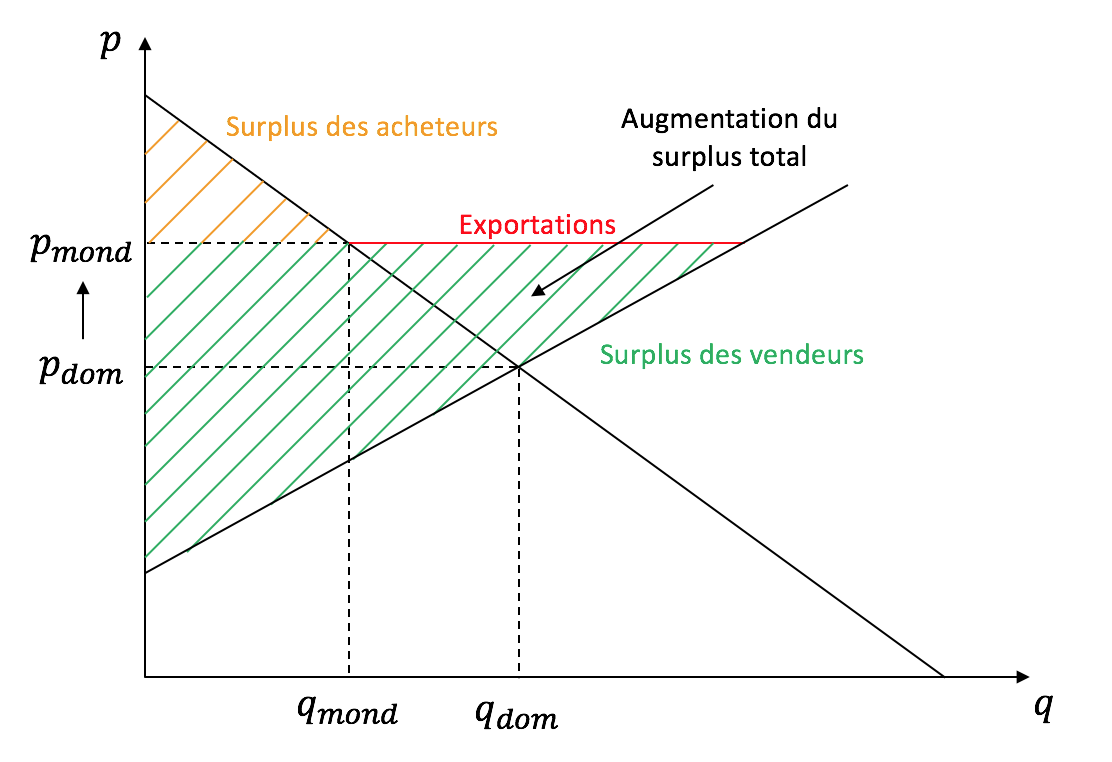
\includegraphics[scale = 0.4]{img/ex.png} & 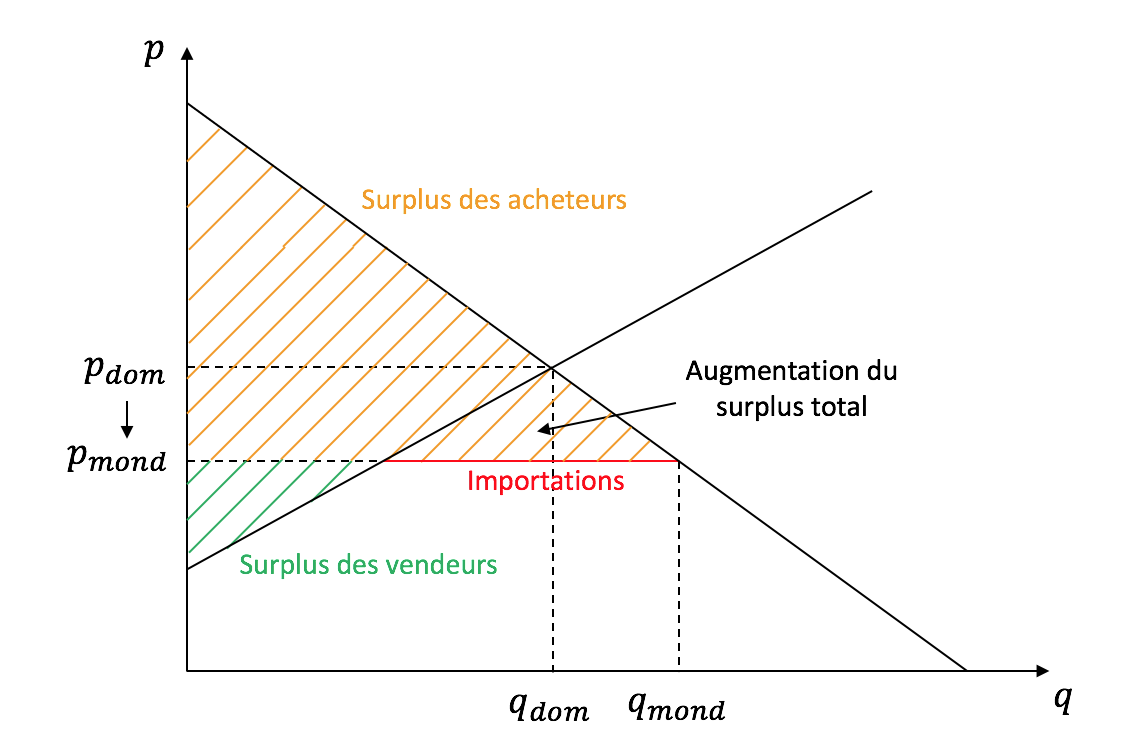
\includegraphics[scale = 0.4]{img/im.png}\\
    Avantage aux producteurs & Avantage aux acheteurs\\
    \hline
    \end{tabular}
\end{table}\\
Dans les deux cas, il y a un gain global à l'ouverture. 
\subsection{Barrières commerciales}
\noindent
L'état peut agir de trois manières différentes sur l'importation et l'exportation de biens.
Il peut introduire une taxe $T$ sur l'importation (cfr. Figure \ref{tim}).
\begin{figure}[ht!]
    \centering
    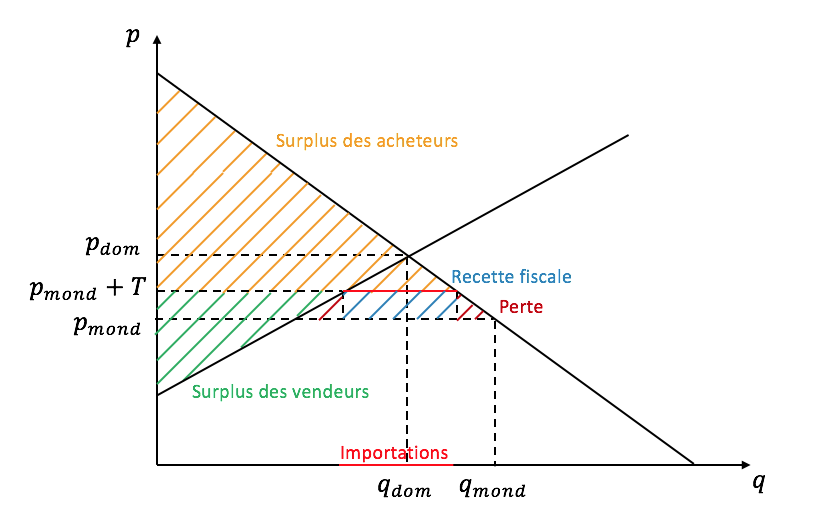
\includegraphics[scale = 1]{img/tim.png}
    \caption{Taxe sur l'importation}
    \label{tim}
\end{figure}\\
\newpage
Il peut mettre un subside $S$ aux exportations (cfr. Figure \ref{sex}). 
\begin{figure}[ht!]
    \centering
    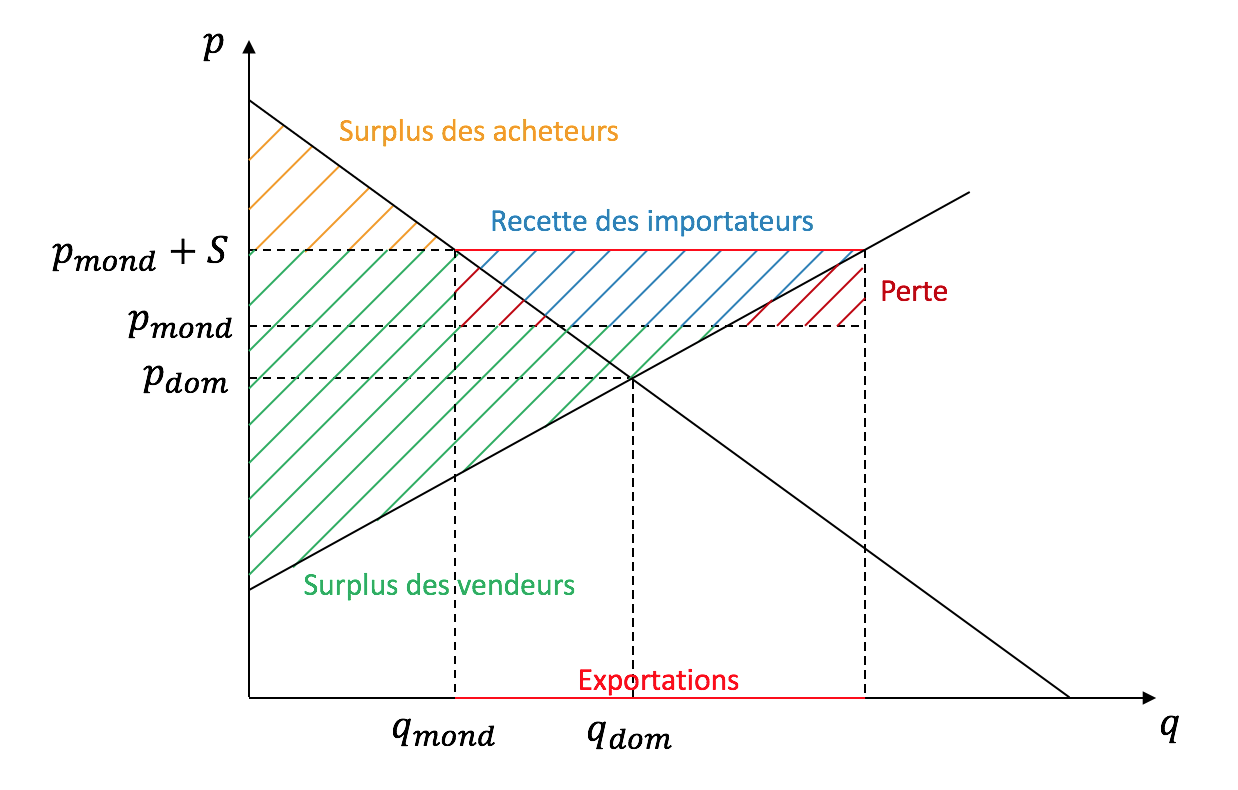
\includegraphics[scale = 0.65]{img/sex.png}
    \caption{Subside sur l'exportation}
    \label{sex}
\end{figure}\\
\newpage
Il peut mettre un quota $Q$ sur les importations (cfr. Figure \ref{qim}). Il limite l'importation des entreprises.
\begin{figure}[ht!]
    \centering
    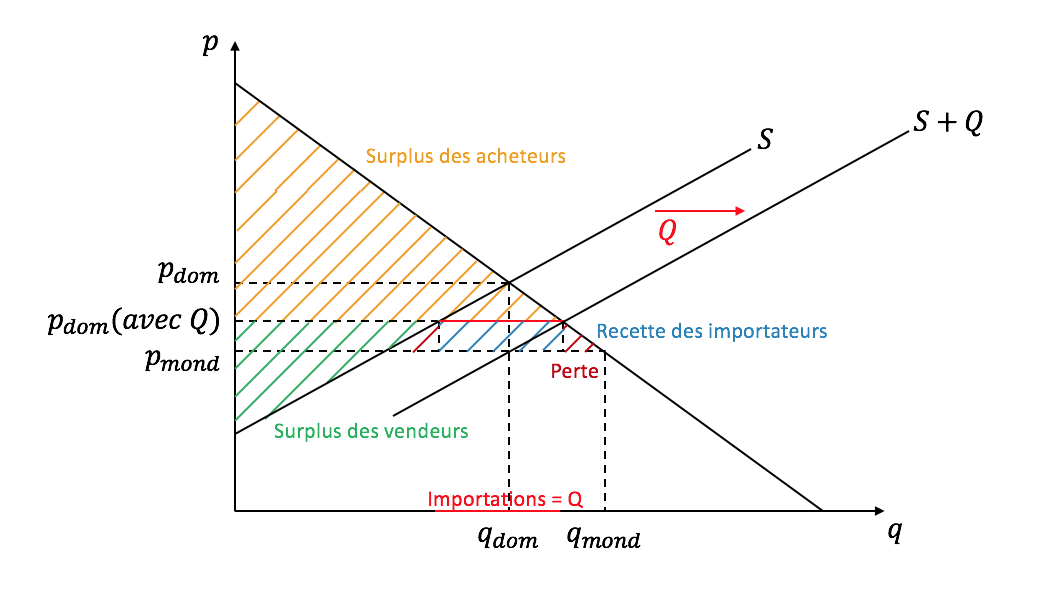
\includegraphics[scale = 0.9]{img/qim.png}
    \caption{Quota sur l'importation}
    \label{qim}
\end{figure}\\
Dans ces trois cas, le surplus des vendeurs va augmenter et on va retrouver une perte globale de surplus supportée par les acheteurs.
\newpage
\part{Macro-économie}
\section{Introduction}
\noindent
La macro-économie est l'étude des effets causés par les décisions de l'ensemble des ménages et des entreprises (pas d'étude individuelle).
Elle se base sur les trois derniers principes de Mankiw. 
\bf{Fonctionnement globale de l'économie} :
\begin{itemize}
\item Le niveau de vie d'un pays dépend de sa capacité à produire des biens et des services.
\item Les prix tendent à augmenter lorsque l'état imprime de la monnaie. Il y a une inflation générale des prix.
\item A court terme, un compromis existe entre l'inflation et le chômage.
\end{itemize}
On distingue deux types d'analyse : 
\begin{itemize}
    \item \bf{L'analyse positive }: On peut confronter les faits entre eux.
    \item \bf{L'analyse normative} : Impossibilité de prouver les faits. On fait des hypothèses.
\end{itemize}
\section{Les indicateurs macro-économiques}
\subsection{La production}
\subsubsection{Le produit intérieur brut}
\noindent
On mesure la production grâce au calcul du produit intérieur brut PIB. Il est défini comme la valeur au marché de tous les biens et services finaux produits dans une économie au cours d'une période donnée.\\
\\
Par conséquent, le PIB ne tient pas compte de 
\begin{itemize}
    \item la valeur des biens intermédiaires (sauf ceux qui sont stockés ou exportés) ;
    \item la valeur de l'économie illégale ou souterraine ;
    \item la valeur des articles produits et consommés non commercialisés ; 
    \item la valeur des biens d'occasion ;
    \item et la valeur des titres financiers.
\end{itemize}
Pour le calculer, on a deux méthodes :  méthode des revenus ou méthode des dépenses. C'est possible grâce à un principe en macro-économie qui dit que 
\[\sum \text{Revenus } = \sum\text{Dépenses}\]
En utilisant la méthode des dépenses, on peut décomposer le PIB en quatre composants.
\[ \text{PIB} = C + I + G + XN\]
où $C$ est la consommation;\\ 
\tab[0.45cm] $I$ est l'investissement;\\
\tab[0.45cm] $G$ sont les dépenses publiques courantes;\\
\tab[0.45cm] $XN$ sont les  importations et les exportations.\\
\\
\subsubsection{Les types de PIB}
\noindent
On distingue deux PIB différents. Tout d'abord, on a le PIB nominal qui est définit par la valeur en prix courants de la production. Son augmentation peut donc être causée par l'augmentation dans les quantités produites ou l'augmentation des prix. Néanmoins, il ne reflète pas fidèlement l'activité économique contrairement au PIB réel. Ce dernier ne varie que si les quantités produites changent. On prend donc une valeur de prix constant fixée dite de référence.
\subsubsection{Le déflateur}
\noindent
Le déflateur mesure le niveau général des prix de toute la production.
\[\text{Déflateur }=\frac{\text{PIB}_\text{nominal}}{\text{PIB}_\text{réel}}*100\]
\subsubsection{Le taux de croissance économique}
\noindent
Le taux de croissance économique mesure l'évolution de la production dans le temps.
\[TC = \frac{\text{PIB}_\text{nominal}(t)-\text{PIB}_\text{nominal}(t-1)}{\text{PIB}_\text{nominal}(t-1)}*100\]
\subsubsection{Le PIB et le bien-être}
\noindent
Le PIB représente la dépense totale d'un pays, et le revenu total de ce pays. Le PIB par habitant représente donc la dépense moyenne et le revenu moyen. On peut donc en conclure que le PIB par habitant est directement corrélé avec le bien-être. Néanmoins, le PIB ne reflète pas tous les aspects du bien-être comme les loisirs, l'environnement, etc. Il est donc sujet à controverse. 
Cependant, un PIB per capita faible est corrélé avec 
\begin{itemize}
    \item un faible niveau d'éducation ;
    \item une espérance de vie courte ; 
    \item et une inégalité des revenus plus importante.
\end{itemize}
\subsection{Le coût de la vie}
\subsubsection{L'indice des prix à la consommation}
\noindent
L'indice des prix à la consommation IPC mesure l'évolution du niveau des prix. Lorsque l'IPC augmente, on a une inflation. L'IPC vaut donc
\[ \text{IPC }= \frac{\text{Coût total du panier d'une année}}{\text{Coût total du panier de l'année de base}}\]
\subsubsection{Le taux d'inflation}
\noindent
Le taux d'inflation est défini comme le taux de croissance de l'IPC.
\[\text{Taux d'inflation } = \frac{\text{IPC}(t)-\text{IPC}(t-1)}{\text{IPC}(t-1)}*100\]
Il faut tenir compte de cette inflation lorsqu'on utilise plusieurs variables qui en sont affectées. Il faut donc faire une conversion si on compare plusieurs variables nominales de différentes années.
\[\text{Variable réelle }=\frac{\text{Variable nominale}}{\text{IPC}}*\text{IPC}_\text{comparaison}\]
\subsection{Le chômage}
\label{chomage}
\noindent
Un chômeur est une personne ayant la capacité de travailler et qui, à la recherche d'un travail rémunéré, se trouve involontairement sans emploi. On retrouve quelques exceptions. Une personne qui est sans emploi mais commence dans quatre semaines au moins ou une personne qui a été mis à pied temporairement depuis six mois au moins peut être considérée comme un chômeur.
On compte trois mesures importantes :
\begin{align*}
    \text{Taux de chômage } & = \frac{\text{Nombre de chômeurs}}{\text{Population active}}*100\\
    \text{Taux d'activité } & = \frac{\text{Nombre de personnes actives}}{\text{Population agée de plus de 16 ans}}*100\\
    \text{Taux d'emploi } & = \frac{\text{Nombre d'emplois}}{\text{Population agée de plus de 16 ans}}*100
\end{align*}
\section{PIB et croissance}
\subsection{Le niveau de vie}
\noindent
Le niveau de vie est directement corrélé avec la croissance puisque le PIB réel par habitant influence directement le revenu moyen par habitant et donc le niveau de vie.\\
Pour pouvoir augmenter le PIB per capita, on retrouve cinq facteurs clés : 
\begin{itemize}
    \item capital physique,
    \item capital humain,
    \item ressources naturelles,
    \item connaissances techniques,
    \item et heures travaillées.
\end{itemize}
\subsection{La productivité}
\noindent
L'efficacité des travailleurs à produire des biens est appelée la productivité du travail. La productivité est le produit par unité de travail. On définit donc la fonction de production comme
\[y = A * f(L,K,H,N)\]
où $A$ sont les connaissances techniques;\\
\tab[0.45cm] $L$ est la quantité de travail;\\
\tab[0.45cm] $K$ est le capital;\\
\tab[0.45cm] $H$ est le capital humain;\\
\tab[0.45cm] $N$ sont les ressources naturelles.\\
Dès lors, on peut définir les rendements marginaux décroissant. Lorsqu'on augmente la quantité d'un facteur de production, le production supplémentaire qui en découle diminue.\\
\\
En économie fermée, on a 
\[y = G+I+C\]
et donc $I = y-C-G$. L'épargne total vaut l'investissement total $S = I$ et on a une accumulation du capital. \\
\subsection{Accumulation du capital}
\noindent
On peut en conclure que pour les pays auxquels le stock du capital est déjà élevé, le capital supplémentaire ne fera pas progresser énormément la productivité. On peut alors définir la notion de rattrapage ; les pays qui démarrent leur trajectoire de croissance en étant pauvres ont tendance à croître plus rapidement que le pays riches.
Il existe cinq facteurs qui permettent la croissance et le développement dans les pays les moins développés PMD.
\begin{itemize}
    \item Liberté économique
    \item Droits de propriété et stabilité politique
    \item Infrastructures de base
    \item Ouverture économique
\end{itemize}
\subsection{Etat stationnaire}
\noindent
L'état stationnaire représente l'équilibre à long terme de l'économie. Le stock de capital par heure-travaillée finit par se stabiliser. L'investissement est égal à l'usure du capital (l'amortissement). Il n'y a donc plus de variation du $K/L$.
\subsection{La croissance de la productivité}
\noindent
Pour un pays pauvre, l'investissement est le moteur de la croissance.\\
Pour un pays avancé, il faut repousser l'état stationnaire en faisant des progrès technologiques ou des progrès dans le capital humain.
Pour permettre une croissance dans les pays avancés, ce dernier doit investir en capital humain et en recherche et développement mais également en accumulant du capital physique. 
\section{Epargne et investissement en économie fermée}
\subsection{Système financier}
\noindent
Le système financier consiste en une série d'institutions qui facilitent les rencontres entre les personnes désirant faire un emprunt et les épargnants. On dit que l'épargnes excédentaire des uns est l'investissement des autres. Toutes ces institutions font parties de groupes qui sont appelé les marchers financiers. On distingue deux grands types d'institutions financières : les banques et les fonds communs de placement. Ces derniers sont des institutions qui vendent des parts au public et consacre les fonds récoltés à l'achat d'un porteuille d'actifs financiers.
\subsection{L'investissement}
\noindent
La décision d'investir découle de critères de décision. Il faut comparer le rendement (flux de revenus nets tiré de l'acquisition de l'actif) du nouveau capital à son coût. Le coût du capital est le coût d'acquisition et d'installation de l'actif.\\
Les entreprises vont investir tant que la valeur actualisée nette est positive (cfr. Section \ref{sec1}).\\
L'investissement dépend également :
\begin{itemize}
    \item des bénéfices nets anticipées des entreprises,
    \item croissance économique, 
    \item du progrès technologique, 
    \item des taxes,
    \item et des subventions.
\end{itemize}
\subsection{L'épargne}
\noindent
On distingue deux types d'épargne : l'épargne privée $S_p = Y-T-C$ et l'épargne publique $S_g = T-G$.
\subsubsection{L'épargne privée}
\noindent
L'épargne privée est le choix entre la consommation présente et la consommation future. Elle dépend de quatre facteurs : 
\begin{itemize}
    \item \bf{Taux de préférence inter-temporelle et taux d'intérêt} : Plus le taux d'intérêt est élevé, plus il vaut la peine de remettre de la consommation à plus tard.
    \item \bf{Revenu disponible} : Plus il y a de revenu disponible, plus on aura tendance à consommer et à épargner.
    \item \bf{Richesse} : Plus on a de richesse, plus on aura tendance à consommer au détriment de l'épargne.
    \item \bf{Revenu futur anticipé} : Plus le revenu anticipé sera élevé, plus on aura tendance à consommer au détriment de l'épargne.
\end{itemize}
\subsubsection{L'épargne publique}
\noindent
L'épargne publique est le solde budgétaire des gouvernements. On a donc une épargne publique positive si on est en surplus budgétaire. 
\subsubsection{L'épargne nationale}
\noindent
L'épargne national est la somme des deux épargnes privée et publique.
\subsection{Le marché des fonds prêtables}
\noindent
\begin{figure}[ht!]
    \centering
    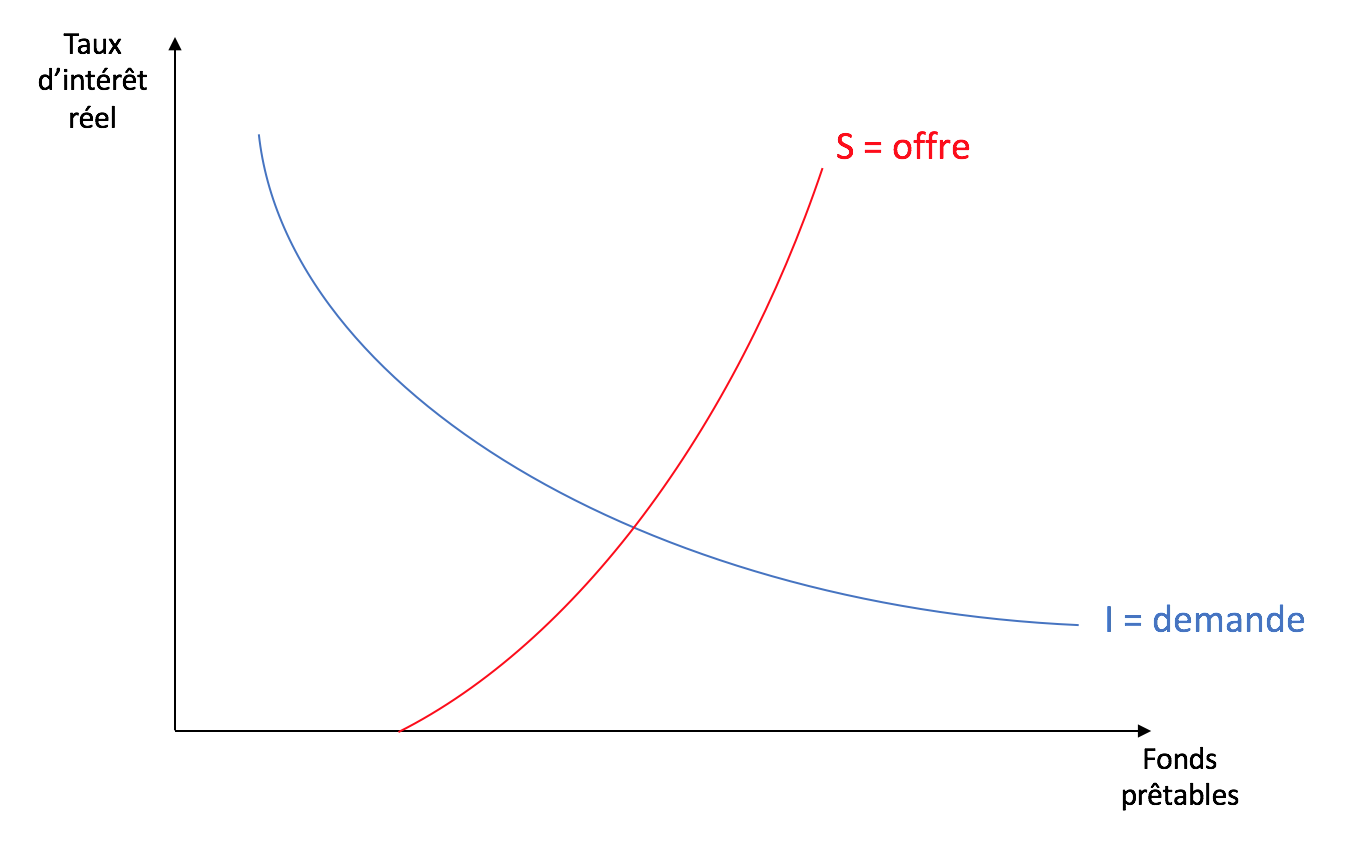
\includegraphics[scale = 0.5]{img/si.png}
    \caption{Les courbes d'offre et de demande}
    \label{si}
\end{figure}\\
\begin{table}[ht!]
    \centering
    \begin{tabular}{|x{8cm}|x{8cm}|}
    \hline
    Incitations à investir &Incitations à épargner \rule[-0.25cm]{0cm}{0.7cm}\\
    \hline
    Hausse des bénéfices anticipés &Hausse du revenu disponible\\
    Réduction des taxes sur les profits & Baisse de la richesse\\
    Hausse des subventions à l'investissement & Baisse du revenu futur anticipé\\
    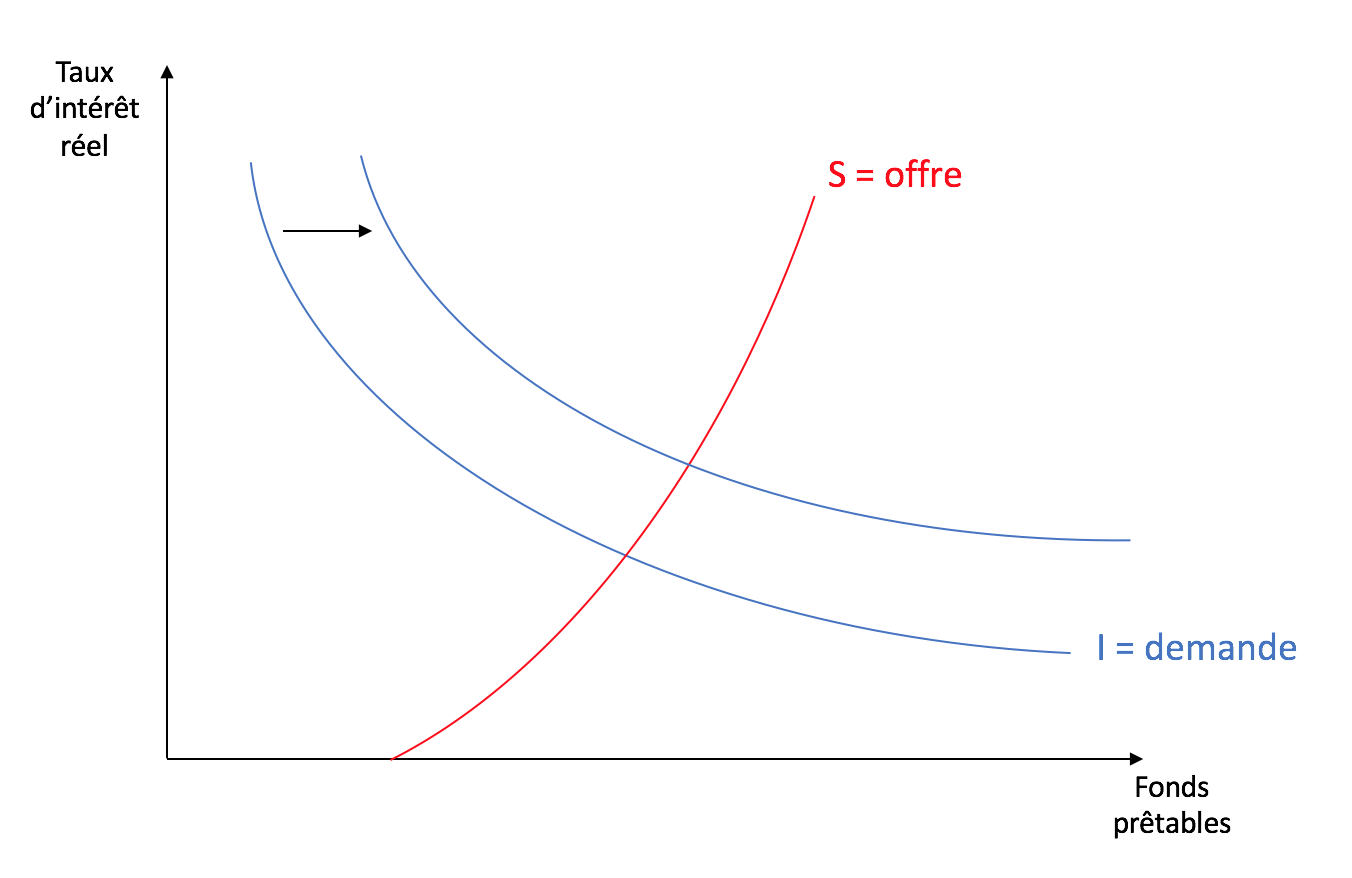
\includegraphics[scale = 0.3]{img/inc1.png} & 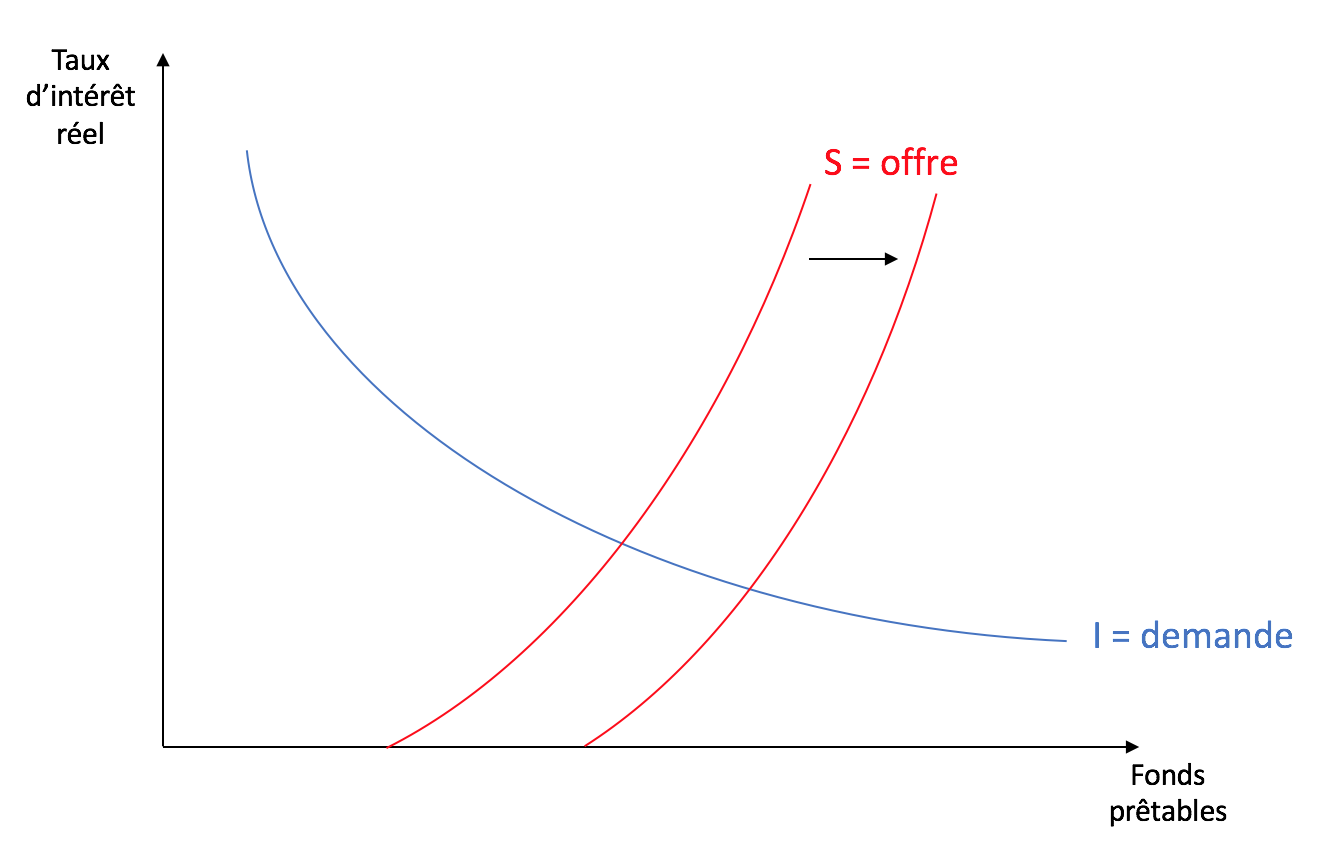
\includegraphics[scale = 0.3]{img/inc2.png}\\
    \hline
    \end{tabular}
\end{table}\\
On retrouve l'effet d'éviction.\\
Si $S_g<0$, on parle de déficit budgétaire. La dette publique augmente et l'offre de fonds prêtables diminue.\\
Si $S_g>0$, on parle de surplus budgétaire.\\
Si le taux d'intérêt augmente, alors les investissements diminuent.
\section{L'économie d'ouverture}
\subsection{Quelques définitions...}
\noindent
Définissons d'abord quelques notions.\\
\bf{Economie ouverte} : est une économie pour laquelle le commerce international se fait librement et prend une part importante dans le produit intérieur brut du pays. \\
\bf{Exportations} : est l'action de vendre à l'étranger une partie de la production de biens ou de services.\\
\bf{Importations} : est une entrée dans un pays de biens ou services provenant d' un autre pays.\\
\bf{Exportations nettes} ou \bf{Balance commerciale} : sont la valeur des exportations moins la valeur des importations. Si exportations $>$ importations, on a un excédent de la balance commerciale. Si exportations $<$ importations, on a un déficit de la balance commerciale. Enfin si exportations $=$ importations, on a un équilibre de la balance commerciale.
\subsection{Les exportations et les importations}
\noindent
Les exportations et les importations sont sujets à variations. Les déterminants de ces variations sont entre autres : les goûts des consommateurs, les prix, les taux de change, les coûts de transport, les politiques commerciales ou les revenus.
\subsubsection{Les flux de capitaux}
\noindent
Les flux de capitaux sont définis par le fait que les résidents d'un pays participent aux marchés financiers mondiaux. On a que les sorties nettes de capitaux SNC valent l'acquisition d'actifs étrangers par des belges moins l'acquisition d'actifs belges par des étrangers ou SNC $=($AAEB$-$AABE$)=$ XN. Il faut toujours que XN et SNC soient égaux. Si une entreprise belge vend un bien à l'étranger, alors XN$\uparrow$.
\subsection{L'épargne et l'investissement}
\noindent
En économie ouverte, on a que $y = C+I+G+XN$, et par conséquent que $S =I+XN$. Mais on sait maintenant que $XN = SNC$. On peut donc écrire que $S = I +SNC$.\\
Une unité épargnée peut servir à acheter des biens d'investissement ici ou à acheter des actifs à l'étranger.
\subsection{Le prix des transactions commerciales}
\subsubsection{Le taux de change nominal}
\noindent
Le taux de change nominal $e$ est le taux auquel on peut échanger une monnaie contre une autre. On peut alors définir deux notions importantes.\\
\bf{L'appréciation} d'une devise : est lorsque son pouvoir d'achat augmente.\\
\bf{La dépréciation} d'une devise : est lorsque son pouvoir d'achat diminue.\\
\subsubsection{Le taux de change réel}
\noindent
Le taux de change réel $E$ est le taux auquel on peut échanger des biens et des services d'un pays contre ceux d'un autre pays.
\[E = \frac{e*\text{prix en Belgique $(P)$}}{\text{Prix à l'étranger $(P\text{*})$}}\]
Les taux de change réels sont importants car ils déterminent les XN.
\begin{itemize}
    \item Si $\uparrow$E (appréciation de l'euro) $\Rightarrow$ nos produits sont relativement plus coûteux $\Rightarrow$ $\downarrow$EX et $\uparrow$IM.\\
    \item Si $\downarrow$E (dépréciation de l'euro) $\Rightarrow$ nos produits sont relativement plus bon marchés $\Rightarrow$ $\uparrow$EX et $\downarrow$IM.\\
\end{itemize}
\subsection{La parité des pouvoirs d'achat}
\noindent
La parité des pouvoirs d'achat PPA est une théorie de la détermination des taux de change. Le taux de change nominal $e$ pour les monnaies de deux pays est lié au prix dans chacun de ces deux pays. Dès lors, $E =1$ et nous avons
\[e = \frac{P\text{*}}{P}\]
Par conséquent, le taux de change doit s'ajuster pour refléter les différences entre les niveaux de prix.
\[\Delta \%e\approx\pi\text{*}-\pi\]
Le PPA n'est pas une théorie parfaite. Certains produits ne sont pas échangeables. Même les biens échangeables ne sont pas de parfaits substituts.
\subsection{L'offre et la demande}
\noindent
En économie ouverte, l'offre de fonds prêtables provient de l'épargne locale $S$. La demande fonds prêtables vient de l'investissement local $I$ et à l'étranger SNC.
\subsection{Le taux d'intérêt}
\noindent
Dans un modèle d'économie ouverte à long terme, on a que le taux d'intérêt est donné et est égal à la somme du taux mondial $r\text{*}$ et de la prime de risque. 
\[r = r\text{*}+\theta\]
Par simplification, on dit que $\theta=0$. Donc, $r=r\text{*}$. Le taux d'intérêt n'égalise donc plus $S$ et $I$. \\
Si le taux mondial $r\text{*}$ est plus élevé que le taux en économie fermée, l'offre est plus élevée que la demande et donc $S>I$ $\Rightarrow$ SNC $>0$.\\
Si le taux mondial $r\text{*}$ est plus faible que le taux en économie fermée, l'offre est plus faible que la demande et donc $S<I$ $\Rightarrow$ SNC $<0$.\\
\\
SNC est déterminé par la différence entre l'offre intérieure de fonds prêtables $S$ et la demande intérieure de fonds prêtables $I$, au taux d'intérêt mondial. Sans oublier que la définition est applicable aux exportations nettes puisque SNC $=$ XN.
\section{Le taux naturel de chômage}
\noindent
Les définitions et les taux ont été définis à la Section \ref{chomage}. Nous les redéfinirons donc pas. 
On distingue deux types de chômage : 
\begin{itemize}
    \item \bf{Chômage frictionnel} : est le temps normal de recherche d'un emploi. Il est généralement causé par un changement soudain. C'est un chômage de court terme.
    \item \bf{Chômage structurel} : est un chômage chronique qui traduit un déséquilibre profond et durable du marché du travail. Il prolonge la durée du chômage actuel. Il est donc causé par des facteurs qui ne permettent pas au marché du travail de trouver un point d'équilibre. Ce chômage se produit, par exemple, lorsque les salaires sont supérieurs au niveau d'équilibre. C'est un chômage de long terme.
\end{itemize}
Le marché du travail semble être statique. Mais en réalité, il y a de fortes créations et destructions d'emploi. Le marché du travail est très flexible.\\
\\
On définit donc le taux de chômage naturel comme le taux vers lequel l'économie tend à long terme ou comme la somme des chômages frictionnel et structurel.\\
On définit également le chômage cyclique ou conjoncturel comme l'écart du chômage par rapport au niveau naturel. Cet écart est créé par des fluctuations économiques de court terme.
\section{La monnaie}
\subsection{Type de monnaie}
\noindent
On distingue deux types de monnaie.
\begin{itemize}
    \item \bf{La monnaie marchandise} : Une marchandise qui a une valeur intrinsèque.
    \item \bf{La monnaie fiduciaire} : La monnaie qui n’a pas de valeur intrinsèque instituée par l'Etat et/ou la loi.
\end{itemize}
\subsection{Fonctions de la monnaie}
\noindent
On distingue trois fonctions de la monnaie.
\begin{itemize}
    \item \bf{Instrument d'échange} : Avec le troc, chaque transaction nécessite la double coïncidence des besoins. L'introduction de la monnaie a facilité les transactions et augmenté le volume du commerce.  L’introduction de la monnaie fiduciaire a augmenté le volume du commerce international.
    \item \bf{Unité de compte} : est une unité standardisée qui permet de mesurer la valeur des biens et des services.
    \item \bf{Une réserve de valeur} : On  peut utiliser la monnaie pour transférer des ressources et du pouvoir d’achat vers l’avenir.
\end{itemize}
\subsection{La politique monétaire}
\noindent
La Banque Centrale BC a pour objectif de contrôler la politique de régulation de la masse monétaire. Elle n’a qu’une influence indirecte sur l’offre de monnaie. \\
Elle achète des actifs et ainsi augmente la quantité de monnaie dans le système bancaire et elle fait opérations sur le marché des changes.\\
\subsection{La théorie classique}
\noindent
L’offre de monnaie est une variable exogène de notre système. La demande de monnaie reflète la part de la richesse que les individus veulent détenir sous forme liquide. \\
On distingue deux types de variable.
\begin{itemize}
    \item \bf{Variables nominales} : mesurées en unités monétaires.
    \item \bf{Variables réelles} : mesurées en unités physiques. Elles ne sont pas influencées par le système monétaire.
\end{itemize}
On peut introduire le principe de neutralité monétaire qui veut que si on double la quantité de monnaie, les prix doublent, mais les variables réelles restent constantes.
\subsection{La théorie quantitative}
\noindent
La théorie quantitative est formalisée à partir d'une équation de conservation de la quantité de monnaie échangée dans l'ensemble des transactions.
\[M*V = P*Y\]
où $M$ est la quantité de monnaie en circulation dans une économie pendant une période donnée;\\
\tab[0.45cm] $V$ est la vitesse de circulation de la monnaie;\\
\tab[0.45cm] $P$  est le niveau des prix;\\
\tab[0.45cm] $Y$ est la production d'une économie pendant une période donnée.\\
A long terme, $V$ est stable et $Y$ ne dépend pas de $M$. Donc, si $\uparrow M$ alors $\uparrow P$
\subsection{L'effet Fisher}
\noindent
L'effet Fisher a pour objectif de mettre en relation le taux d'intérêt nominal $i$ et le taux d'intérêt réel $r$.
\[i \approx r+\pi\]
À long terme, une augmentation de la quantité de monnaie n’a aucun effet sur $r$. On parle de neutralité monétaire. Mais à court terme, les prix des biens et des services sont fixes. En conclusion, une politique monétaire expansionniste peut avoir des effets sur le taux réel.\\
\\
Si la BC augmente la quantité de monnaie et que les prix des biens et des services restent fixes, alors la production doit augmenter et le chômage diminuer. $\downarrow i$ $\Rightarrow$ $\downarrow r$, ce qui entrainera une augmentation de $C$ et de $I$.\\
\\
Si $i=0$, la politique monétaire ne parvient plus à stimuler l'économie. On ne peut pas avoir de $i<0$, pour stimuler $r$.

\end{document}
